\documentclass[12pt,a4paper]{book}

% Formato del documento
%\usepackage[papersize={210mm,297mm},inner=3.5cm,outer=2cm,top=2.5cm,bottom=2.5cm]{geometry}
%\renewcommand{\baselinestretch}{1}
%\setlength{\parskip}{8pt}

\usepackage[T1]{fontenc}
\usepackage[spanish]{babel}
\usepackage{lmodern}

\usepackage[utf8]{inputenc}


\usepackage{amssymb}
\usepackage{amsmath}
\usepackage{graphicx}
\usepackage{tikz}
\usepackage{tkz-graph}
\usepackage[parfill]{parskip}
\usepackage{float}
\usepackage{subcaption}
\usepackage{multirow} 

\usepackage{algorithm}
\usepackage[noend]{algpseudocode}

\usepackage[natbibapa]{apacite}
\usepackage{hyperref}

\renewcommand{\chaptername}{Capítulo}
\renewcommand{\contentsname}{Índice}
\renewcommand{\bibname}{Bibliografía}
\renewcommand{\figurename}{Figura}
\definecolor{verde_oscuro}{rgb}{0.0, 0.5, 0.0}

\newtheorem{defi}{Definición}[section]
\newtheorem{prop}{Proposición}[section]
\newtheorem{propi}{Propiedades}[section]
\newtheorem{lema}{Lema}[section]
\newtheorem{tma}{Teorema}[section]
\newtheorem{cor}{Corolario}[section]
\newtheorem{nota}{Nota}[section]
\newtheorem{ejem}{Ejemplo}[section]

\addto\captionsspanish{%
  \renewcommand{\tablename}{Tabla}%
}

\hypersetup{
    colorlinks=true,
    linkcolor=blue,
    filecolor=magenta,      
    urlcolor=cyan,
    pdftitle={Overleaf Example},
    pdfpagemode=FullScreen,
    }

\urlstyle{same}

%%%%%%%ALTERNATIVA 2%%%%%%%%%%%%
\textheight=21cm
\textwidth=17cm
%\topmargin=-1cm
\oddsidemargin=0cm
\evensidemargin=0cm
\parindent=0mm
\pagestyle{plain}
%%%%%%%%%%%%%%%%%%%%%

%%%%%%%  Comando Portada  %%%%%%%%%%%
% Ajustes de geometría si la portada sigue sin caber
% \geometry{a4paper, top=1cm, bottom=1cm, left=1cm, right=1cm} 

\newcommand{\nuevaportada}[6]{
    \thispagestyle{empty}
    \begin{center}
        % Usamos \vfill para empujar el contenido hacia abajo desde el borde superior
        \vfill 
        
        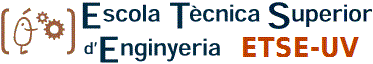
\includegraphics[width=0.45\textwidth]{images/logo.png}
        
        \vspace{0.5cm} % Un espacio fijo pequeño
        {\large\bfseries\textsc{M\'aster Universitario en #1}\par} % Reducido a \large
        
        \vspace{0.5cm}
        
\includegraphics[width=0.35\textwidth]{images/uv.png} % Imagen ligeramente más pequeña
        
        \vspace{0.5cm}
        {\large\bfseries\textsc{Trabajo de Fin de M\'aster}\par} % Reducido a \large
        
        % \vfill distribuye el espacio restante entre este punto y el siguiente
        \vfill 
        
        {\LARGE\bfseries #2\par} % Mantenemos el título principal en \LARGE
        
        \vfill % Otro espacio elástico
        
        \begin{flushright}
            \begin{tabular}{l} 
                {\large\bfseries\textsc{Autor:}} \\
                {\large\textsc{#3}} \\ [0.2cm] % Espacio reducido
                {\large\bfseries\textsc{Tutora:}} \\ 
                {\large\textsc{#4}} \\ [0.2cm] % Espacio reducido
                {\large\bfseries #5} 
            \end{tabular}
        \end{flushright}
        
        \vfill % Espacio final para empujar el bloque de autor hacia arriba
    \end{center}
}

\begin{document}

\nuevaportada{Ciencia de Datos}{Resolución mediante \textit{GRASP} y Aprendizaje Reforzado del Problema Multiobjetivo de Localización de k-Centros Balanceado }{Manuel Rubio Martínez}{Anna Martínez Gavara}{Septiembre, 2025}

\clearpage

\newpage
\tableofcontents

\newpage

\section*{Resumen}
En este Trabajo de Fin de Máster se aborda el problema de localización multiobjetivo de $k$-centros balanceados. Dicho problema surge como una extensión del clásico problema de localización de $k$-centros, en el que, además de minimizar las distancias entre usuarios e instalaciones, se introduce la necesidad de balancear la carga asignada a cada centro. Este equilibrio resulta de gran interés en aplicaciones reales, como la ubicación de hospitales, almacenes o centros de distribución, donde no solo importa la accesibilidad sino también una adecuada distribución de la demanda.

El problema ha sido objeto de estudio reciente en la literatura. En \cite{k-balanced_1}, los autores formulan por primera vez el problema de $k$-centros balanceado y proponen un algoritmo evolutivo denominado \textit{MOAkBCL}, inspirado en el conocido \textit{NSGA-II \citep{NSGA-II}}. Posteriormente, en \cite{k-Balanced_2}, se desarrolla un nuevo enfoque basado en metaheurísticas de tipo \textit{GRASP} \citep{GRASP}, enriquecida con técnicas de Oscilación Estratégica \citep{oscillation} y Path Relinking \citep{path_relinking}, con el fin de explorar de forma más eficiente el espacio de búsqueda y mejorar la calidad de las soluciones.

En este trabajo se propone una nueva aproximación al problema, combinando la metaheurística \textit{GRASP} con técnicas de Aprendizaje Reforzado. El objetivo es aprovechar la capacidad adaptativa del aprendizaje automático para guiar el proceso de búsqueda y generar soluciones de mayor calidad, extendiendo así los trabajos previos con un enfoque distinto. 

Para validar los resultados del algoritmo, se realizarán experimentos con tiempos parecidos a los realizados en ambos artículos. El lenguaje de programación en el que se ha desarrollado el trabajo es Python, considerablemente más lento que el lenguaje del primer artículo, C\#, o el del segundo, Java. No obstante, se han corrido en un ordenador con especificaciones mejores a los 2 artículos previos. Todo esto se tendrá en cuenta en la parte experimental.
\newpage

\section*{Abstract}
In this Master's Thesis, we address the multi-objective balanced $k$-center location problem. This problem arises as an extension of the classical $k$-center location problem, where, in addition to minimizing the distances between users and facilities, the need to balance the load assigned to each center is introduced. This balance is of great interest in real-world applications, such as the location of hospitals, warehouses, or distribution centers, where not only accessibility but also an adequate distribution of demand is important.

The problem has recently attracted attention in the literature. In \cite{k-balanced_1}, the authors first formulate the balanced $k$-center problem and propose an evolutionary algorithm called \textit{MOAkBCL}, inspired by the well-known \textit{NSGA-II \citep{NSGA-II}}. Subsequently, in \cite{k-Balanced_2}, a new approach based on \textit{GRASP} metaheuristics \citep{GRASP}, enriched with Strategic Oscillation techniques \citep{oscillation} and Path Relinking \citep{path_relinking}, was developed in order to explore the search space more efficiently and improve solution quality.

In this work, we propose a new approach to the problem by combining the \textit{GRASP} metaheuristic with Reinforcement Learning techniques. The objective is to exploit the adaptive capabilities of machine learning to guide the search process and generate higher-quality solutions, thereby extending previous works with a different perspective.

To validate the results of the algorithm, experiments will be conducted with execution times comparable to those reported in both articles. The programming language used for the implementation is Python, which is considerably slower than the language used in the first article, C\#, or that of the second, Java. Nevertheless, the experiments have been run on a computer with better specifications than those in the two previous studies. All these factors will be taken into account in the experimental section.

\newpage

\section*{Resum}
En aquest Treball de Fi de Màster s'aborda el problema de localització multiobjectiu de $k$-centres balancejats. Aquest problema sorgeix com una extensió del clàssic problema de localització de $k$-centres, en el qual, a més de minimitzar les distàncies entre usuaris i instal·lacions, s'introdueix la necessitat de balancejar la càrrega assignada a cada centre. Aquest equilibri resulta de gran interés en aplicacions reals, com la ubicació d'hospitals, magatzems o centres de distribució, on no sols importa l'accessibilitat sinó també una adequada distribució de la demanda.

El problema ha sigut objecte d'estudi recent en la literatura. En \cite{k-balanced_1}, els autors formulen per primera vegada el problema de $k$-centres balancejat i proposen un algorisme evolutiu denominat \textit{MOAkBCL}, inspirat en el conegut \textit{NSGA-II \citep{NSGA-II}}. Posteriorment, en \cite{k-Balanced_2}, es desenvolupa un nou enfocament basat en metaheurístiques de tipus \textit{GRASP} \citep{GRASP}, enriquida amb tècniques d'Oscil·lació Estratègica \citep{oscillation} i Path Relinking \citep{path_relinking}, amb la finalitat d'explorar de forma més eficient l'espai de cerca i millorar la qualitat de les solucions.

En aquest treball es proposa una nova aproximació al problema, combinant la metaheurística \textit{GRASP} amb tècniques d'Aprenentatge Reforçat. L'objectiu és aprofitar la capacitat adaptativa de l'aprenentatge automàtic per a guiar el procés de cerca i generar solucions de major qualitat, estenent així els treballs previs amb un enfocament distint.

Per a validar els resultats de l'algorisme, es realitzaran experiments amb temps semblants als realitzats en tots dos articles. El llenguatge de programació en el qual s'ha desenvolupat el treball és Python, considerablement més lent que el llenguatge del primer article, C\#, o el del segon, Java. No obstant això, s'han corregut en un ordinador amb especificacions millors als 2 articles previs. Tot això es tindrà en compte en la part experimental.
\newpage
 
\chapter{Introducción}

El origen de la optimización se remonta a la antigua Grecia, donde matemáticos como Euclides o Arquímedes la utilizaban en busca de soluciones a problemas del área de la geometría.

La versión que conocemos hoy en día no empezó a desarrollarse hasta el siglo XVII, con la aparición del cálculo diferencial \citep{calculo_diferencial}, impulsado por los trabajos de Isaac Newton y Gottfried Wilhelm Leibniz \citep{Leibniz}. Con él se pudieron estudiar las funciones y sus puntos extremos,
en los cuales, bajo ciertas condiciones, pueden encontrarse sus valores óptimos.

No aparecen grandes avances hasta mediados del siglo XX cuando, fruto de la necesidad de resolver problemas logísticos durante la Segunda Guerra Mundial, el matemático George Bernard Dantzig \citep{Dantzig} desarrolló la programación lineal, que sentó las bases para el posterior surgimiento tanto de la programación no lineal, como de la entera y la dinámica.

A pesar de todo, la mayoría de problemas del mundo real, especialmente aquellos que dependen de un gran número de variables, con funciones objetivo complejas y restricciones no lineales, acaban siendo demasiado costosos computacionalmente. Esta inviabilidad de los métodos de obtención de soluciones exactas propició el surgimiento de los metaheurísticos.

Los algoritmos metaheurísticos \citep{metaheuristicos}, acuñados por el especialista en ciencias de la computación Fred Glover,
son la alternativa realista para la búsqueda de soluciones aproximadas, pero cercanas al óptimo, en un tiempo aceptable.

Las metaheurísticas son fundamentales en Ciencia de Datos, ya que permiten abordar de manera eficiente problemas complejos presentes en:

\begin{itemize}
    \item \textbf{Clustering:} El algoritmo \textit{k-means} \citep{k-means} particiona el espacio de observaciones en un número determinado de clústeres (grupos) y determina qué observaciones pertenecen a cada uno de ellos. 
    Si intentásemos encontrar la solución exacta, sería computacionalmente muy costoso, y la naturaleza del algoritmo hace que la solución sea dependiente de los grupos iniciales (generados aleatoriamente), pudiendo caer una y otra vez en los mismos \textbf{óptimos locales} (ver en \ref{def:optimo_local}).
    Las metaheurísticas ayudan a solventar estos problemas al proporcionar estrategias más robustas de exploración del espacio de soluciones.
    
    \item \textbf{Selección de variables:} En la construcción de modelos de predicción, solemos encontrarnos con un número elevado de variables, por lo que definir el modelo con base en todas ellas no es factible. Mediante metaheurísticos podemos 
    reducir significativamente la dimensión del espacio, utilizando un subespacio con las variables que mejor sirvan al modelo.
    
    \item \textbf{Ajuste de hiperparámetros:} Modelos de inteligencia artificial como las redes neuronales necesitan ajustar multitud de hiperparámetros para ser eficaces (número de capas, tasa de aprendizaje, etc.). Este ajuste constituye también un problema de optimización en espacios de búsqueda de alta dimensión, frente a métodos tradicionales como la búsqueda en cuadrícula (\textit{grid search}), los metaheurísticos ofrecen una alternativa más eficiente y flexible. En el artículo \cite{hyperparameters} se puede ver el ejemplo de uso.
\end{itemize}

En esencia, la optimización es el proceso de encontrar las mejores soluciones para un problema determinado, de la forma más eficiente y precisa posible.
Cualquier reto que se enmarque en esta búsqueda de un resultado óptimo puede considerarse, por tanto, un problema de optimización.

Si bien esta idea es intuitiva, el rigor matemático exige una definición más precisa.

\section{Formulación Matemática}

Para expresar un problema de optimización de forma matemática, definimos las tres partes en las que se puede descomponer:

\begin{itemize}
    \item \textbf{Variables de Decisión:} Son las incógnitas del problema, los valores que deberemos modificar para obtener la solución o soluciones óptimas. Se representan como un vector $\mathbf{x} = (x_1, x_2, \ldots, x_n)$, donde $n$ es el número de variables.

    \item \textbf{Función Objetivo:} Función que se desea minimizar o maximizar.
    Se denota comúnmente como $f(\mathbf{x})$, donde $f$ es la función que establece la relación entre las variables ($\mathbf{x}$) y el objetivo que deseamos optimizar.
    Por ejemplo:
    $$ \min_{\mathbf{x}} f(\mathbf{x}) \quad \text{o} \quad \max_{\mathbf{x}} f(\mathbf{x}) .$$
    La función $f: \mathbb{R}^n \to \mathbb{R}$ mapea el vector de variables a un valor escalar, el cual buscaremos mejorar.

    \item \textbf{Restricciones:} Son las condiciones o limitaciones que deben satisfacer las variables de decisión. Pueden ser de igualdad o de desigualdad. Se expresan generalmente como:
    \begin{align*}
        g_i(\mathbf{x}) &\le 0 & \quad \text{para } i = 1, \ldots, m \\
        h_j(\mathbf{x}) &= 0 & \quad \text{para } j = 1, \ldots, p
    \end{align*}
    Donde $g_i(\mathbf{x})$ son las $m$ restricciones de desigualdad y $h_j(\mathbf{x})$ son las $p$ restricciones de igualdad.
    En caso de tener restricciones del tipo $g_k(\mathbf{x})\geq0$, se puede transformar a $\leq$ sabiendo que $-g_k(\mathbf{x}) \leq 0$.
    
    Además de restricciones funcionales, también pueden existir restricciones sobre el \textbf{dominio} (ver en \ref{def:dominio}) de sus variables, como $x_k \ge 0$ (variables no negativas),  $x_k \in \{0,1\}$ (variables binarias) o $x_k \in \mathbb{Z}$ (variables enteras).
\end{itemize}

Ahora sí, pasadas las definiciones previas, un problema completo de optimización se formula de la siguiente manera:
$$
\begin{array}{ll}
\text{Minimizar (o Maximizar)} & f(\mathbf{x}) \\ \\
\text{Sujeto a:} & g_i(\mathbf{x}) \le 0, \quad i = 1, \ldots, m \\
& h_j(\mathbf{x}) = 0, \quad j = 1, \ldots, p \\
& \mathbf{x} \in X
\end{array}
$$
Donde $X$ representa el conjunto de factibilidad o dominio de las variables de decisión.

En el siguiente apartado se van a clasificar los problemas de optimización según dos características principales.

\subsection{Optimización Lineal vs. No Lineal}

La primera distinción la haremos según la naturaleza de las funciones involucradas, tanto en la función objetivo como en las restricciones.

\subsubsection{Optimización Lineal}
Diremos que un problema es de \textbf{optimización lineal} cuando, tanto la función objetivo como todas las funciones de las restricciones, son \textbf{lineales} (ver en \ref{def:f_lineal}) con respecto a las variables de decisión. 

La optimización lineal se caracteriza por:
\begin{itemize}
    \item La función objetivo tiene la forma $f(\mathbf{x})=c_1x_1+c_2x_2+...+c_nx_n$ donde los $c_i \in \mathbb{R} \quad \forall i \in 1,2,...,n$.
    \item Todas las restricciones son lineales y tienen el formato $a_1x_1+a_2x_2+...+a_nx_n\leq b$ o $=b$, donde $a_i \in \mathbb{R} \quad \forall i \in 1,2,...,n$ y $b\in \mathbb{R}$.
    \item Estas condiciones hacen que el conjunto de soluciones factibles ($X$) sea semejante a un poliedro \textbf{convexo} (ver en \ref{def:convexo}), lo que simplifica la búsqueda de la solución óptima.
    \item El algoritmo Simplex, propuesto en \cite{Dantzig1951}, es el más extendido para resolver este tipo de problemas y garantiza encontrar el \textbf{óptimo global} (ver en \ref{def:optimo_global}), si existe.
\end{itemize}

\subsubsection{Optimización No Lineal}
Diremos que un problema es de \textbf{optimización no lineal} cuando al menos una de sus funciones (objetivo o de restricción) es no lineal (con respecto a sus variables de decisión). 

Las características principales de la optimización no lineal son:
\begin{itemize}
    \item La función objetivo $f(\mathbf{x})$ o alguna de sus restricciones $g_i(\mathbf{x})$ o $h_j(\mathbf{x})$ contiene términos no lineales. Por ejemplo:
    $$f(\mathbf{x})=2x_1^2+5x_2^7-\ln(x).$$
    \item El conjunto de soluciones factibles puede ser no convexo, lo que deriva en múltiples óptimos locales y el aumento de la complejidad del problema a la hora de buscar el óptimo global.
    \item La mayoría de algoritmos para resolverlos suelen utilizar técnicas de búsqueda local y no garantizan encontrar el óptimo global.
\end{itemize}

Ejemplos:
\begin{itemize}
    \item \textbf{Lineal:} Una fábrica busca maximizar su beneficio produciendo varios artículos, donde cada uno consume una cantidad fija de recursos (horas de máquina, materia prima) y genera un beneficio fijo, con restricciones de recursos y uso de las máquinas.
    \item \textbf{No lineal:} Encontrar los parámetros de una curva que se ajustan a unos datos concretos, minimizando el error cuadrático medio entre la aproximación (la curva) y el valor exacto de los datos.
\end{itemize}


\subsection{Optimización Discreta vs. Continua}
La segunda característica a estudiar será la naturaleza de sus variables de decisión. Que sean continuas o discretas
limitará en gran medida el tipo de algoritmos que puedan utilizarse para resolverlos.

\subsubsection{Optimización Continua}
En la optimización continua, las variables de decisión pueden tomar cualquier valor real dentro de su dominio o rango permitido. Es decir, no están restringidas a tomar valores enteros, a un conjunto finito o a un conjunto \textbf{numerable} (ver en \ref{def:conjunto_numerable}) de posibles soluciones. Esto las hace adecuadas para modelar fenómenos que varían de forma suave, como el tiempo, el espacio, la temperatura, etc.

Características principales:
\begin{itemize}
    \item Variables pertenecientes a un espacio continuo, típicamente $\mathbb{R}^n$.
    \item Las funciones objetivo $f(\mathbf{x})$ y sus restricciones $g_i(\mathbf{x}), \;h_j(\mathbf{x})$ suelen ser \textbf{continuas} y \textbf{diferenciables} (ver en \ref{def:fun_continua} y en \ref{def:fun_diferenciable}).
    \item Las técnicas de resolución a menudo involucran cálculo diferencial para encontrar el mejor camino de mejora de la solución.
\end{itemize}

\subsubsection{Optimización Discreta}
En este caso, las variables de decisión sí están restringidas a tomar valores en un conjunto finito o numerable. Los casos más comunes son variables restringidas a tomar valores enteros $(0,1,2,...)$, binarios $(0,1)$ o variables que representan la elección de elementos de un conjunto específico (por ejemplo, el ``trabajador 1'' o el ``trabajador 2'').

Características principales:
\begin{itemize}
    \item Las variables pertenecen al espacio discreto.
    \item No se pueden utilizar directamente las técnicas de cálculo diferencial que, en cambio, sí se podrían usar en el espacio continuo.
    \item Los problemas suelen ser más complejos de resolver y computacionalmente más costosos, por lo que suelen requerir algoritmos específicos como la programación entera \citep{int_programing}, la programación dinámica o métodos combinatorios para poder resolverlos.
\end{itemize}

Ejemplos:
\begin{itemize}
    \item \textbf{Continuos:} El diseño de la aerodinámica de un avión (modelado de los parámetros de las curvas de la superficie) o la velocidad óptima de un vehículo para reducir su consumo de combustible.
    \item \textbf{Discretos:} El problema de la mochila (escoger el mayor valor en elementos de un conjunto sin exceder una capacidad dada) o por qué lugares pasa un camión en la planificación de rutas.
\end{itemize}

Para esta primera parte de caracterización de la optimización se ha tomado como referencia el libro \textit{Numerical Optimization} de \cite{Numerical_optimization_nocedal_wright}. 

Para concluir la parte teórica de la optimización, se va a concretar tanto la rama a la que pertenece el problema multiobjetivo de k-centros balanceado (la optimización \textbf{combinatoria}) como lo que significa que sea \textbf{multiobjetivo}.

\subsection{Optimización Combinatoria}
La optimización combinatoria se centra en encontrar la solución óptima dentro de un conjunto de soluciones finito o numerable. Aunque la cantidad de soluciones posibles pueda ser finita, no significa que el problema sea sencillo.
De hecho, la mayoría de estos problemas de optimización entran dentro de los denominados problemas \textbf{NP-difíciles} \citep{np_hard}.

Que sean NP-difíciles implica que el tiempo necesario para encontrar la solución óptima crece exponencialmente a medida que aumenta el tamaño del problema. Esto hace que la búsqueda exhaustiva de la solución sea computacionalmente inviable para la mayoría de los casos de estudio en el mundo real.

Sus características principales son las siguientes:
\begin{itemize}
    \item \textbf{Espacio de soluciones discreto:} Las variables de decisión están restringidas a un conjunto finito o numerable de valores, como la selección o no de un elemento, o la ordenación de un conjunto. Entran dentro de los casos de \textbf{optimización discreta}. 
    \item \textbf{Complejidad computacional elevada:} A menudo, el número de soluciones posibles es astronómicamente grande, lo que requiere algoritmos especializados para explorar el espacio de búsqueda de manera eficiente.
    \item \textbf{Estructura del problema:} Las técnicas de resolución aprovechan la estructura combinatoria subyacente del problema, utilizando métodos como la programación entera, la teoría de grafos o los algoritmos metaheurísticos.
\end{itemize}

Algunos ejemplos clásicos de optimización combinatoria incluyen el \textbf{Problema del Viajante de Comercio (TSP)}, 
que busca la ruta más corta que visita un conjunto de ciudades una sola vez;
el \textbf{Problema de la Mochila}, que consiste en seleccionar los objetos más valiosos sin superar una capacidad de peso;
o la \textbf{planificación de horarios}, donde se asignan recursos (como aulas o profesores) a franjas horarias para satisfacer un conjunto de restricciones.

\subsection{Optimización Multiobjetivo}

Definir la cantidad de funciones objetivo que se van a utilizar para modelizar el problema constituye una de las características más relevantes y, a menudo, más complejas del mismo, debido a su naturaleza inherentemente subjetiva.
¿Debe considerarse únicamente una función objetivo? ¿Hay que tener en cuenta simultáneamente 
dos o más funciones objetivo? Si bien enfocarse en una única función facilita el análisis y su resolución, rara vez refleja la complejidad de los problemas reales. La optimización multiobjetivo
abordará los problemas mejorando simultáneamente dos o más funciones objetivo que, a menudo, estarán en conflicto entre sí. Mejorar una suele implicar el empeoramiento de la otra.

Por ejemplo, en el diseño de un vehículo, minimizar el consumo de combustible (objetivo 1) estará en conflicto con maximizar la potencia del motor (objetivo 2).

La optimización multiobjetivo permite abordar este tipo de situaciones analizando
explícitamente las compensaciones o \textit{trade-offs} entre los diferentes objetivos. En lugar de proporcionar una única solución, esta técnica ofrece un conjunto de soluciones eficientes y equilibradas que permiten
tomar decisiones evaluando distintas alternativas y elegir la que mejor se adapte a las necesidades del problema.

En este contexto, el concepto de “solución óptima” deja de ser aplicable. En su lugar, se busca identificar un conjunto de soluciones que representen las mejores compensaciones posibles entre los objetivos. Este conjunto se denomina \textbf{Frente de Pareto}.

Una solución se considera \textbf{no dominada} (u óptima en el sentido de Pareto) si no existe otra solución factible que la supere en al menos un objetivo sin empeorar en ninguno de los demás. El Frente de Pareto está compuesto por todas las soluciones no dominadas del espacio de soluciones factibles.
\begin{figure}[H]
    \centering
    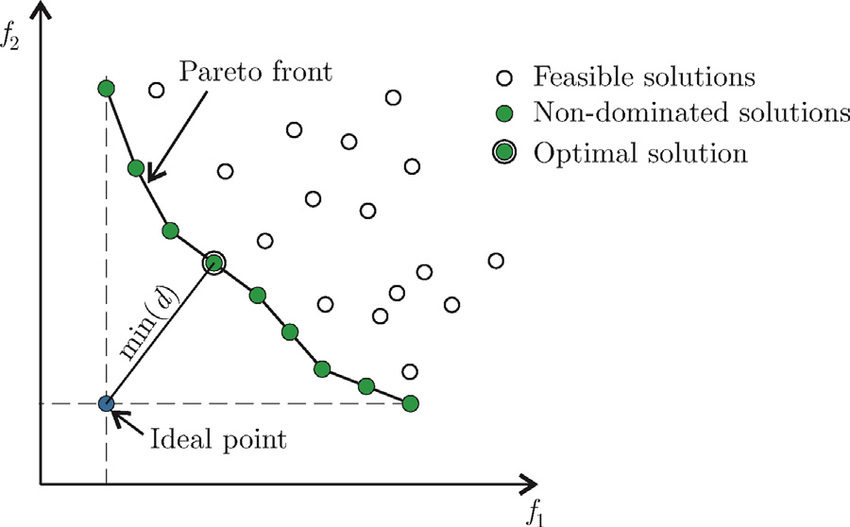
\includegraphics[width=0.6\textwidth]{images/pareto_front.png}
    \caption{\citep{Bre2017} Ilustración de un Frente de Pareto para un problema de minimización con dos objetivos ($f_1, f_2$).}
    \label{fig:pareto}
\end{figure}
Las soluciones en verde son óptimas y pertenecen al Frente de Pareto, ya que no se puede mejorar un objetivo sin empeorar el otro. El punto ideal, que estaría en la parte inferior izquierda de la gráfica, sería la mejor solución imaginable combinando lo mejor de todas las soluciones. Las soluciones sin colorear están dominadas por alguna de las verdes.

Una vez definidos los problemas de optimización, se pueden enunciar las dos maneras que hay de resolverlos.

\section{Resolución de Problemas de Optimización Multiobjetivo}

\subsection{Métodos Exactos}

Los métodos exactos para la optimización multiobjetivo tienen como finalidad encontrar el Frente de Pareto al completo. Sin embargo, al igual que en sus contrapartes monoobjetivo, se enfrentan al mismo obstáculo: la complejidad computacional. La mayoría de estos problemas son \textbf{NP-difíciles}.

No obstante, para problemas sencillos, con pocas variables y reducido espacio de soluciones, se pueden resolver con los siguientes métodos:

\begin{itemize}
    \item \textbf{Métodos de Ponderación (\textit{Weighted Sum}):} Transforman el problema multiobjetivo en problemas monoobjetivo, asignando pesos a cada una de las funciones objetivo y sumándolos para crear una única función agregada. Al variar sistemáticamente los pesos, se pueden ir generando las soluciones del Frente de Pareto. Sin embargo, este método no garantiza encontrar todas las soluciones si el frente tiene una forma no convexa.

    \item \textbf{Método de las Restricciones Épsilon (\textit{$\epsilon$-constraint}):} Consiste en optimizar una de las funciones objetivo, convirtiendo el resto en restricciones que limitan su valor a un máximo $\epsilon$.\\
    Modificando los valores de $\epsilon$ para cada objetivo-restricción, se puede explorar y reconstruir el Frente de Pareto. A diferencia del método de ponderación, este sí puede encontrar soluciones en frentes no convexos.

    \item \textbf{Algoritmos de Ramificación y Acotación (\textit{Branch and Bound}) Multiobjetivo:} Estos algoritmos extienden el clásico \textit{Branch and Bound} \citep{bnb}. El proceso de ramificación es similar (se divide el problema en subproblemas más pequeños), pero la fase de acotación (o poda) es más compleja. En lugar de usar una única cota, se trabaja con conjuntos de cotas (un vector por cada objetivo). Una rama del árbol de búsqueda se poda solo si se puede demostrar que no puede contener ninguna solución no dominada en comparación con las soluciones ya encontradas.

    \item \textbf{Algoritmos de Ramificación y Corte (\textit{Branch and Cut}) Multiobjetivo:} De manera análoga, esta técnica extiende \textit{Branch and Cut} \citep{bnc}. Se añaden planos de corte (restricciones adicionales) no solo para mejorar la relajación del problema monoobjetivo, sino para refinar la aproximación del espacio de soluciones factibles en el dominio multiobjetivo, permitiendo podar ramas del árbol de búsqueda de forma más eficiente.
\end{itemize}

\subsection{Metaheurísticas}
Como se indicó al principio del capítulo, las metaheurísticas \citep{metaheuristicos} aparecen con el desarrollo de las ciencias de la computación como principal solución a los problemas de optimización complejos. Allí donde los métodos exactos no son capaces de encontrar el óptimo,
los algoritmos metaheurísticos buscan soluciones ``buenas'' en tiempos de ejecución razonables, sacrificando la garantía de optimalidad global que proporcionan los métodos exactos.

Generalmente combinan heurísticas con aleatoriedad para explorar el espacio de soluciones y obtener resultados diversos, a la vez que se intensifica la búsqueda en las distintas regiones en busca de nuevos óptimos locales. Estos métodos combinan dos estrategias:
\begin{itemize}
    \item \textbf{Exploración:} Capacidad de recorrer diversas áreas del espacio de búsqueda para encontrar nuevas soluciones, evitando quedar atrapado en óptimos locales.
    \item \textbf{Explotación:} Capacidad de intensificar la búsqueda en una región prometedora para encontrar los mejores óptimos locales dentro de ella.
\end{itemize}

Son algoritmos muy generales y se adaptan a casi cualquier problema de optimización. Algunos de los principales algoritmos metaheurísticos son:
\begin{itemize}
    \item \textbf{Algoritmos Genéticos (\textit{GA - Genetic Algorithms}):}
    Inspirados en la selección natural y la genética, se basan en la generación aleatoria de soluciones y en el cruce de las más prometedoras entre sí, 
    mientras se añaden mutaciones (pequeñas modificaciones en las soluciones) para aportar diversidad.
    
    \item \textbf{Recocido Simulado (\textit{SA - Simulated Annealing}):}
    Basado en un proceso físico, simula el recocido de metales (calentarlos y enfriarlos para alterar su estructura). Explora soluciones aceptando movimientos de mejora, pero también aquellos que puedan empeorar la solución, 
    en función de una probabilidad dependiente de una variable ``temperatura'', que decrece con el paso de las iteraciones. En fases tempranas, una temperatura alta favorece la exploración, mientras que en fases finales una temperatura baja favorece la explotación.
    
    \item \textbf{Búsqueda Tabú (\textit{TS - Tabu Search}):}
    Genera una lista ``tabú'' que actúa como memoria a corto plazo del algoritmo, incluyendo los movimientos recientes con el objetivo de no repetir soluciones y así forzar la exploración de nuevas zonas, aunque eso conlleve aceptar movimientos que no sean los mejores posibles.
    
    \item \textbf{Optimización por Colonia de Hormigas (\textit{ACO - Ant Colony Optimization}):}
    Diseñado originalmente para problemas de rutas, construye soluciones iterativamente a través de un grafo, cuyas aristas se van ponderando a medida que se generan soluciones de calidad.
    
    \item \textbf{\textit{GRASP} (\textit{Greedy Randomized Adaptive Search Procedure}):}
    Algoritmo fundamentado en dos fases. Una primera de construcción, en la que se genera una solución mediante un proceso aleatorizado, y una segunda de búsqueda local, en la que se intenta mejorar la solución generada.
\end{itemize}

\section{Aprendizaje Reforzado}

El Aprendizaje Reforzado \citep{intro_reforzado} (del inglés, \textit{Reinforcement Learning} o RL) es un área del aprendizaje automático inspirada en la psicología conductista. Se utiliza en problemas donde un agente debe tomar acciones en un entorno dinámico con el objetivo de maximizar una cierta recompensa.

A diferencia de otros paradigmas de la ciencia de datos como el aprendizaje supervisado, donde los algoritmos aprenden de un conjunto de datos etiquetado, en RL el agente aprende por sí mismo a través de la experiencia directa, en un proceso de prueba y error. 

El objetivo del RL no es encontrar la respuesta correcta, sino descubrir una estrategia de actuación óptima que maximice la recompensa a largo plazo. Por esta razón, el RL se considera un problema de optimización secuencial de decisiones.

El agente busca optimizar su comportamiento para lograr un objetivo a largo plazo, lo que lo convierte en una herramienta excepcionalmente potente para resolver problemas complejos en dominios como la robótica, la gestión de la cadena de suministro, las finanzas algorítmicas o incluso para resolver los propios problemas de optimización combinatoria.

\subsection{Componentes Clave del Aprendizaje Reforzado}

Todo problema de Aprendizaje Reforzado se modela a través de los siguientes elementos:

\begin{itemize}
    \item \textbf{Agente}: Entidad que aprende del entorno y toma las decisiones. Puede ser un robot que aprende a caminar, un programa que juega al ajedrez o un sistema de gestión de tráfico urbano.
    \item \textbf{Entorno}: Es el mundo, real o simulado, donde se encuentra e interactúa el agente. Este únicamente puede tener control parcial del entorno.
    \item \textbf{Tiempo ($T$)}: Momentos discretos en los que se desarrolla el Aprendizaje Reforzado ($t=0, 1, 2, \dots$).
    \item \textbf{Estado ($S$)}: Descripción de la situación del entorno. Representa toda la información relevante que el agente puede necesitar para la toma de decisiones. $S_t$ representa el entorno en el momento $t$.
    \item \textbf{Acción ($A$)}: Es el conjunto de las posibles decisiones que el agente puede tomar. $A_t$ representa la acción tomada en el momento $t$.
    \item \textbf{Recompensa ($R$)}: Señal numérica que el entorno devuelve al agente tras cada acción. La recompensa indica cómo de buena o mala ha sido la acción tomada al transitar al nuevo estado $S_{t+1}$. El objetivo del agente es maximizar la suma de estas recompensas a lo largo del tiempo. $R_t$ es la recompensa obtenida en el momento $t$.
\end{itemize}

El proceso de aprendizaje se desarrollaría de la siguiente manera:
\begin{enumerate}
    \item El agente observa el estado actual del entorno, $S_t$.
    \item Basándose en $S_t$, el agente elige una acción, $A_t$.
    \item El entorno recibe la acción $A_t$ y, como resultado, transita a un nuevo estado, $S_{t+1}$.
    \item El entorno emite una recompensa, $R_{t+1}$, al agente.
\end{enumerate}
Este ciclo iterativo genera una trayectoria de estados, acciones y recompensas que el agente utilizará para aprender estrategia que maximice su rendimiento a largo plazo.

El objetivo del agente no es maximizar la recompensa inmediata, sino el \textbf{retorno} (o recompensa acumulada), denotado como $G_t$.
El retorno es la suma de todas las recompensas futuras a partir del instante $t$. 
Para evitar sumas infinitas en tareas continuas y para dar más importancia a las recompensas cercanas en el tiempo, se introduce un factor de descuento $\gamma$, donde $0 \le \gamma \le 1$.

El \textbf{retorno descontado} se define como:
\[ G_t = R_{t+1} + \gamma R_{t+2} + \gamma^2 R_{t+3} + \dots = \sum_{k=0}^{\infty} \gamma^k R_{t+k+1} .\]

\begin{itemize}
    \item Si $\gamma = 0$, el agente solo tiene en cuenta la recompensa inmediata.
    \item Si $\gamma$ se acerca a 1, el agente valora las recompensas futuras casi tanto como las inmediatas.
\end{itemize}

El problema de optimización en RL consiste en encontrar una estrategia que maximice el valor esperado de este retorno. Para encontrarla, volvemos a tener el dilema que encontramos a la 
hora de definir las metaheurísticas.

\subsection{Exploración vs. Explotación}

Para que un agente aprenda la manera  óptima qué acciones tomar, deberá equilibrar la explotación y la exploración:
\begin{itemize}
    \item \textbf{Explotación}: Utilizar el conocimiento actual para tomar la mejor acción conocida y maximizar la recompensa inmediata.
    \item \textbf{Exploración}: Probar nuevas acciones, potencialmente subóptimas, para descubrir si pueden conducir a recompensas mayores a largo plazo y mejorar su conocimiento del entorno.
\end{itemize}
Si únicamente explota, se arriesga a quedar atascado en un óptimo local.
Si solo explora, obtendrá un rendimiento bajo al no aprovechar las buenas acciones que ha descubierto previamente.

El dilema se suele solventar siguiendo una estrategia \textbf{$\epsilon$-greedy (épsilon-voraz)}, donde el agente elige la mejor acción conocida con probabilidad $1-\epsilon$ (explotación) y una acción aleatoria con probabilidad $\epsilon$ (exploración).

\subsection{Ejemplos de Aplicación del Aprendizaje Reforzado}

\subsubsection{El Problema del Bandido de múltiples brazos (\textit{Multi-Armed Bandit})}

El problema del \textit{Multi-Armed Bandit} (\textit{MAB}) \citep{MAB} es un ejemplo clásico que ilustra perfectamente el dilema de exploración vs. explotación. Imaginemos a un jugador en un casino frente a $k$ máquinas tragaperras (los ``bandidos'').
Cada máquina $i$ tiene una probabilidad desconocida $p_i$ de dar una recompensa. El objetivo del jugador es maximizar su ganancia total en un número limitado de jugadas.

\begin{itemize}
    \item \textbf{Agente}: El jugador.
    \item \textbf{Acciones}: Elegir una de las $k$ máquinas para jugar.
    \item \textbf{Recompensa}: 1 si la máquina da premio, 0 si no.
    \item \textbf{Estado}: En su formulación más simple, este problema no tiene diferentes estados, ya que la decisión sobre qué máquina jugar no depende de una configuración previa del entorno.
\end{itemize}

¿Debería el jugador seguir jugando con la máquina que, hasta ahora, ha dado los mejores resultados (explotación), o debería probar otras máquinas que podrían tener una tasa de pago aún mayor (exploración)?

Una solución siguiendo la política $\epsilon$-greedy sería:
\begin{enumerate}
    \item Estimar el valor esperado para cada una de las máquinas en $A$ (la recompensa media obtenida por cada una de ellas).
    \item Con probabilidad $1-\epsilon$, elegir la máquina $A_i \in A$ que haya generado una mayor recompensa media.
    \item Con probabilidad $\epsilon$, elegir una máquina al azar.
\end{enumerate}

Este sistema se suele utilizar en ensayos clínicos para asignar pacientes a diferentes tratamientos.

\subsubsection{Juegos de Estrategia}

Se utiliza incluso en juegos de estrategia complejos como el ajedrez, Go o videojuegos.

\begin{itemize}
    \item \textbf{Agente}: El programa que juega.
    \item \textbf{Estado}: La configuración actual del tablero o la pantalla del juego.
    \item \textbf{Acciones}: Los movimientos legales de las piezas o los comandos del mando.
    \item \textbf{Recompensa}: +1 por ganar la partida, -1 por perder y 0 por cada movimiento que no termine la partida.
\end{itemize}

Sistemas como AlphaGo \citep{AlphaGo} de DeepMind utilizaron RL para aprender a jugar a Go a un nivel sobrehumano.
El agente juega millones de partidas contra sí mismo, explorando el espacio de estrategias y entrenando una función de valor que le permita evaluar la calidad de cualquier posición del tablero.


\section{Resumen de los capítulos}
El presente Trabajo de Fin de Máster se estructura en cinco capítulos, además de un anexo con definiciones necesarias para entender el trabajo, y las referencias utilizadas.

En el capítulo 2 se presenta el Problema de Localización de k-Centros Balanceado, introduciendo el marco general de los problemas de localización, la motivación de este estudio y el modelo matemático para resolverlo.

El capítulo 3 expone la justificación de la elección de la metaheurística \textit{GRASP} para abordar el problema, describe su implementación y detalla la incorporación del Aprendizaje Reforzado, mediante \textit{Multi-Armed Bandits} (\textit{MAB}).

El capítulo 4 recoge el diseño experimental y el análisis de los resultados obtenidos, comparando el rendimiento del algoritmo \textit{GRASP} con y sin refuerzo frente a soluciones reportadas en estudios previos.

Finalmente, el capítulo 5 presenta las conclusiones derivadas del trabajo, así como posibles líneas de investigación futura.

\chapter{Problema Multiobjetivo de Localización de k-Centros Balanceado}

\section{Problemas de Localización de instalaciones}

Los \textbf{problemas de localización de instalaciones} (\textit{Facility Location Problems} en su terminología en inglés) constituyen una de las clases más relevantes dentro de la optimización combinatoria. Su objetivo es determinar las \textbf{ubicaciones óptimas} donde instalar infraestructuras como almacenes, hospitales, escuelas o antenas de telecomunicaciones.

Suelen centrarse en:
\begin{itemize}
    \item \textbf{Minimizar los costes} o las distancias (ya sea la distancia total o la máxima entre instalaciones y clientes).
    \item \textbf{Maximizar beneficios} o el área de cobertura alcanzada.
    \item \textbf{Mejorar la equidad} del servicio o los tiempos de respuesta.
    \item \textbf{Equilibrar el uso} entre las distintas instalaciones.
\end{itemize}

Para encontrar la solución óptima, en estos problemas de localización también se deben considerar \textbf{restricciones} prácticas, como la capacidad de cada centro, los límites presupuestarios o la necesidad de cubrir un mínimo de demanda.

Encontrar la solución óptima es vital en \textbf{logística y cadena de suministro}, donde ubicar estratégicamente almacenes y centros
de distribución reduce drásticamente los costes de transporte y mejora la eficiencia de entregas. También en el \textbf{sector sanitario}, en el cual ubicar hospitales y centros de atención primaria es crítico para
asegurar la máxima cobertura y accesibilidad de los mismos a toda la población, o en otros servicios públicos como la \textbf{planificación de escuelas}, \textbf{estaciones de bomberos} o \textbf{ubicación de bocas de metro}.

Algunas de las soluciones propuestas en la literatura se basan en los siguientes modelos:

\subsubsection{P-Mediana (\textit{p-median})}
El objetivo de este modelo es seleccionar $p$ ubicaciones de manera que se \textbf{minimice la suma total de las distancias} entre cada cliente y la instalación que se le asigna. Su enfoque está orientado a optimizar la \textbf{eficiencia global del sistema}, lo que lo convierte en una herramienta idónea para reducir los costes totales de transporte.
Se utiliza, por ejemplo, para determinar la ubicación de almacenes minimizando los costes de distribución, o para ubicar los centros de reciclaje reduciendo la distancia total recorrida por los vehículos de recogida.

\subsubsection{K-Centro (\textit{k-center})}
En este modelo, el objetivo es seleccionar $k$ ubicaciones para \textbf{minimizar la máxima distancia} que cualquier cliente debe recorrer hasta la instalación más cercana. Se trata de un enfoque centrado en la \textbf{equidad}, ya que busca optimizar el ``peor caso''. Es especialmente relevante en el diseño de servicios de respuesta rápida o de carácter crítico.

Su uso es clave en localizar qué hospitales se construyen para que el máximo tiempo de llegada ante una emergencia sea lo menor posible, o al ubicar las estaciones de bomberos, con el objetivo de que puedan responder
en situaciones remotas lo más rápido posible.

\subsubsection{Problemas de Cobertura (\textit{Coverage})} 
Estos modelos tienen como propósito \textbf{maximizar la demanda atendida} dentro de un radio de servicio predefinido. 
Suelen usarse en el diseño de redes de telecomunicaciones, donde cada antena de telefonía móvil cubre un área geográfica determinada.

\begin{itemize}
    \item \textbf{\textit{Location Set Covering Problem} (\textit{LSCP}):}
    Su objetivo es \textbf{minimizar el número de instalaciones} necesarias para cubrir todos los puntos de demanda.
Por ejemplo, se utiliza para determinar el número mínimo de escuelas de forma que todos los estudiantes vivan a menos de 2 km de alguna de ellas.

    \item \textbf{\textit{Maximal Covering Location Problem} (\textit{MCLP}):}
En este caso, el objetivo es \textbf{maximizar la demanda cubierta} con un número fijo de instalaciones, lo que resulta especialmente útil cuando no es posible cubrir a toda la población.
Es necesario para casos en los que se selecciona la ubicación de bibliotecas móviles para dar servicio al mayor número posible de ciudadanos.

\end{itemize}

El \textbf{problema de localización multiobjetivo de k-centros balanceado}: Consiste en seleccionar, de un conjunto de $m$ posibles centros, los $k$ que mejoren sus funciones objetivo:
\begin{itemize}
    \item Minimizar la distancia entre cliente más alejado y su centro más cercano.
    \item Minimizar la carga de trabajo del centro más congestionado.
    \item Reducir la diferencia de cargas entre la instalación más utilizada con respecto a la que menos.
\end{itemize}

\section{Motivación}

En un entorno cada vez más competitivo y dinámico, la localización estratégica de infraestructuras no solo debe considerar criterios tradicionales como la distancia o el coste, sino también otros factores clave como la cobertura del mercado, la accesibilidad o el equilibrio en la distribución de la demanda.

Actualmente, uno de los principales retos es maximizar el alcance de ciertos productos o servicios, garantizando que lleguen al mayor número posible de personas. Al mismo tiempo, es necesario evitar la concentración excesiva de demanda en unos pocos puntos, lo que puede provocar saturación, pérdida de calidad del servicio o ineficiencias operativas, mientras existen centros que, por tener una localización más aislada, prácticamente no recibirían demanda.

El equilibrio entre amplitud de cobertura y uso equilibrado de los recursos disponibles es especialmente importante en contextos donde hay un reducido número de emplazamientos posibles, y donde cada selección de localización afecta tanto a la eficiencia del sistema como a la experiencia del usuario o cliente final.

Al abordar el problema es importante considerar que la distancia total o el tiempo medio de viaje no es el factor más crítico. 
Tomemos como ejemplo la construcción de un hospital en una ciudad: el objetivo no es que la población viva lo más cerca posible, sino que todos los residentes se encuentren a una distancia razonable para poder acceder al servicio.

Considerando estos dos escenarios para la ciudad:

\begin{itemize}
    \item \textbf{Escenario 1}: El tiempo medio de trayecto hasta el hospital más cercano es de 15 minutos, y el tiempo máximo que ha de recorrer un individuo de 30 minutos.
    \item \textbf{Escenario 2}: El tiempo medio de trayecto hasta el hospital más cercano es de 13 minutos, pero pasa a 1 h el tiempo que tendrá de recorrer la persona más alejada de su hospital más cercano.
\end{itemize} 

En términos globales, se podría decir que el segundo sistema implementado es más eficiente, pero se dejan de lado los valores extremos.
Una parte significativa de la población podría tener grandes dificultades para acceder a servicios esenciales.
Por el contrario, aunque el primer caso tenga un tiempo medio mayor, mejora considerablemente la accesibilidad. Esto subraya que mejorar la media no implica necesariamente mejora el servicio.
\newpage

Para ilustrar estas ideas de forma práctica, consideremos un ejemplo ficticio inspirado en la zona de Valencia, donde una red hospitalaria está
planificando la ubicación de 5 centros médicos dentro de una región con una población de $1000$ personas. 

Debido a limitaciones presupuestarias, de personal e infraestructura, se restringe su construcción a un conjunto de $50$ posibles emplazamientos. 

El objetivo será encontrar qué $5$ centros, de ese total de $50$ posibles, habrá que construir teniendo en cuenta los siguientes criterios:

\begin{itemize}
    \item \textbf{Cobertura Poblacional:} Los centros seleccionados deben intentar minimizar la máxima distancia o tiempo de viaje entre el conjunto de la población y los centros médicos.
    \item \textbf{Capacidad:} Los centros médicos no deben quedar sobresaturados. Construir un único centro médico en una zona con mucha población puede generar una buena cobertura y tiempos de viaje cortos, pero quedar sobrepasado y generar problemas de tiempo de atención y espera.
    \item \textbf{Equilibrio:} Si se construye un centro, tiene que utilizarse. No puede ocurrir que un centro quede muy poco usado con respecto a los demás. Por tanto, otro objetivo será que la diferencia entre los más usados y los menos sea la mínima posible, quedando las cargas bien repartidas.
\end{itemize}

% Con respecto a la imagen, mas o menos hay una tasa de 6.25,  1 unidad equivaldrá a 6 metros.

En la Figura~\ref{fig:centros_medicos} se muestra la distribución inicial, donde 1000 puntos azules representan a la población y 50 estrellas rojas indican las posibles ubicaciones de los centros médicos.

A continuación, se presentan tres soluciones de ejemplo:

\begin{itemize}
    \item \textbf{Solución aleatoria (Figura~\ref{fig:solucion_aleatoria}):} En esta solución cuatro de los centros se ubican en la periferia, mientras el restante permanece en el centro, lo que genera sobrecarga en esta instalación y deja a varios puntos muy alejados de cualquier centro médico (hasta 3.13 km). En este caso, el centro más cargado atiende a 417 personas, mientras que el menos utilizado solo a 49.
    \item \textbf{Solución de cobertura poblacional (Figura~\ref{fig:min_distancias}):} Aquí se busca minimizar la distancia máxima de la población a los centros. La distancia máxima se reduce a 2.35 km, pero se genera un desequilibrio significativo en la carga de los centros, donde el más utilizado atiende a 281 personas y el menos a 69. Tanto esta solución como la siguiente, han sido encontradas
    utilizando el algoritmo propuesto en este trabajo.
    \item \textbf{Solución equilibrada (Figura~\ref{fig:equilibrada}):} Esta alternativa prioriza distribuir de manera equitativa la demanda entre los centros. El centro más utilizado atiende a 203 personas y el menos a 197. Sin embargo, la distancia máxima supera ligeramente los 3 km.
\end{itemize}



\begin{figure}[H]
    \centering
    \begin{subfigure}{0.48\textwidth}
        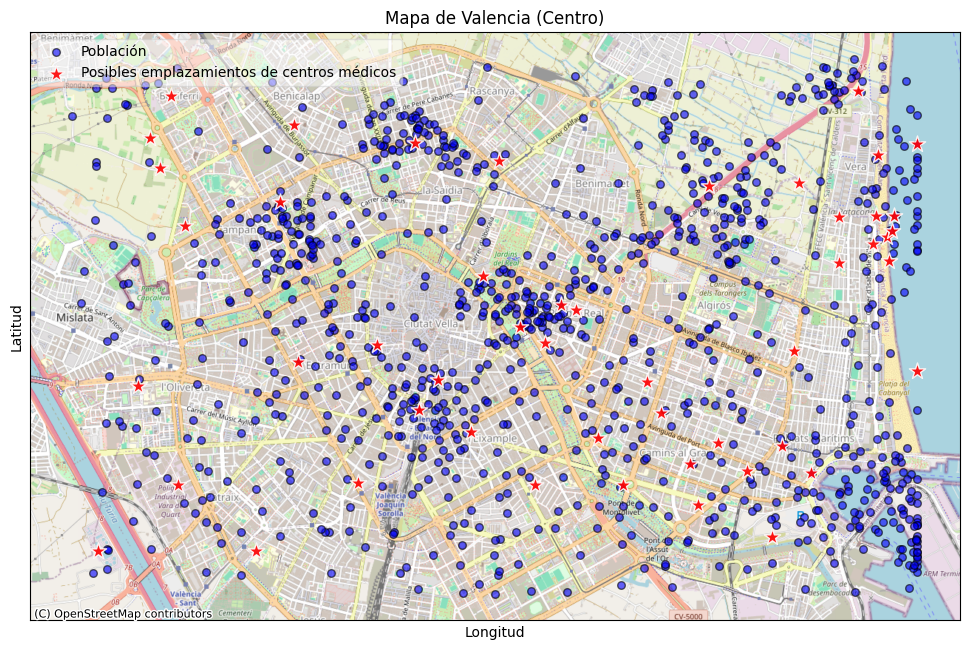
\includegraphics[width=\textwidth]{images/centros_medicos.png}
        \caption{Población y centros médicos potenciales.}
        \label{fig:centros_medicos}
    \end{subfigure}
    \hfill
    \begin{subfigure}{0.48\textwidth}
        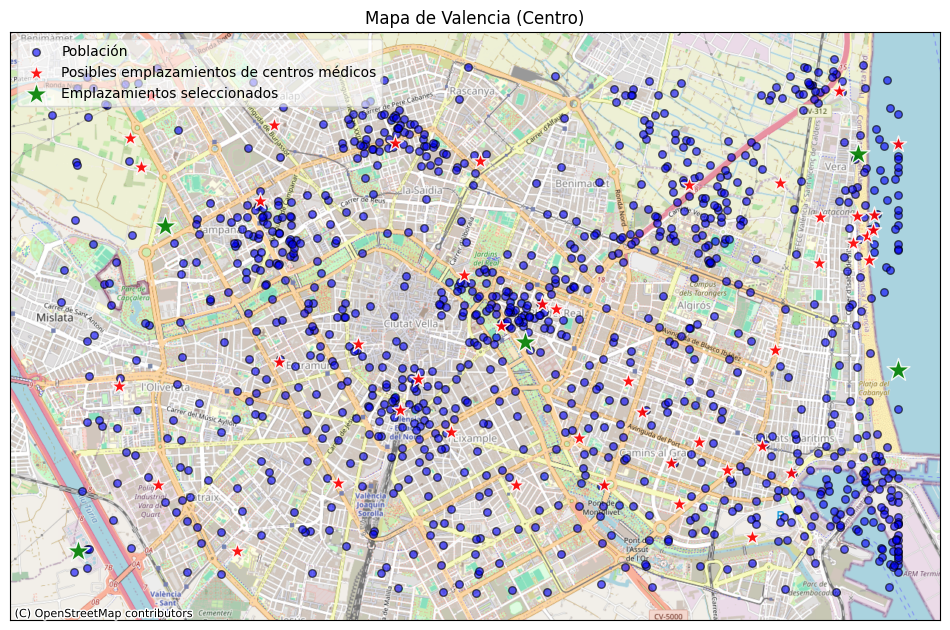
\includegraphics[width=\textwidth]{images/solucion_aleatoria.png}
        \caption{Solución aleatoria.}
        \label{fig:solucion_aleatoria}
    \end{subfigure}
    
    \vspace{0.5cm} % Espacio vertical entre las filas de imágenes
    
    \begin{subfigure}{0.48\textwidth}
        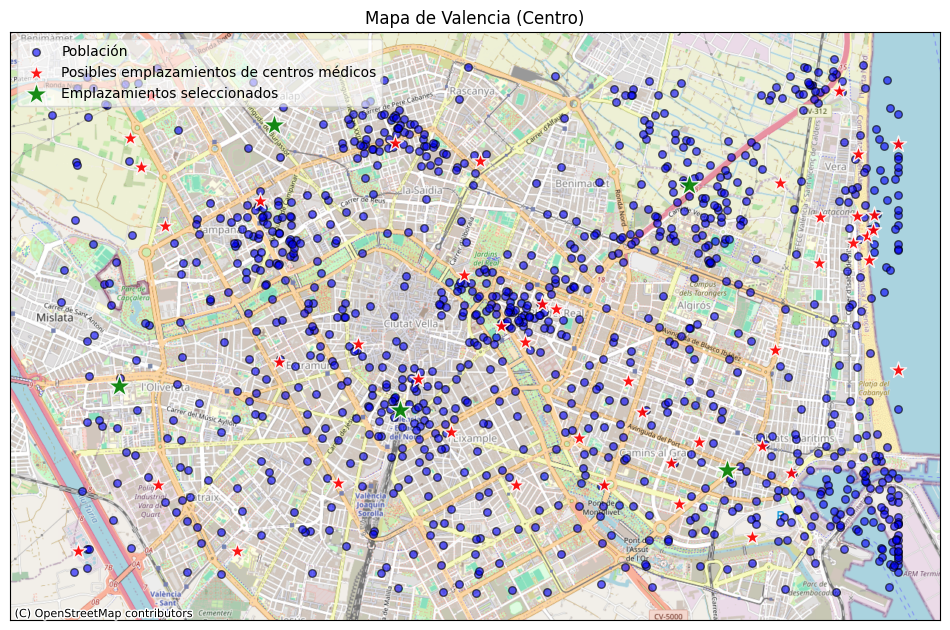
\includegraphics[width=\textwidth]{images/min_distancias.png}
        \caption{Solución encontrada por el algoritmo, minimizando distancia máxima.}
        \label{fig:min_distancias}
    \end{subfigure}
    \hfill
    \begin{subfigure}{0.48\textwidth}
        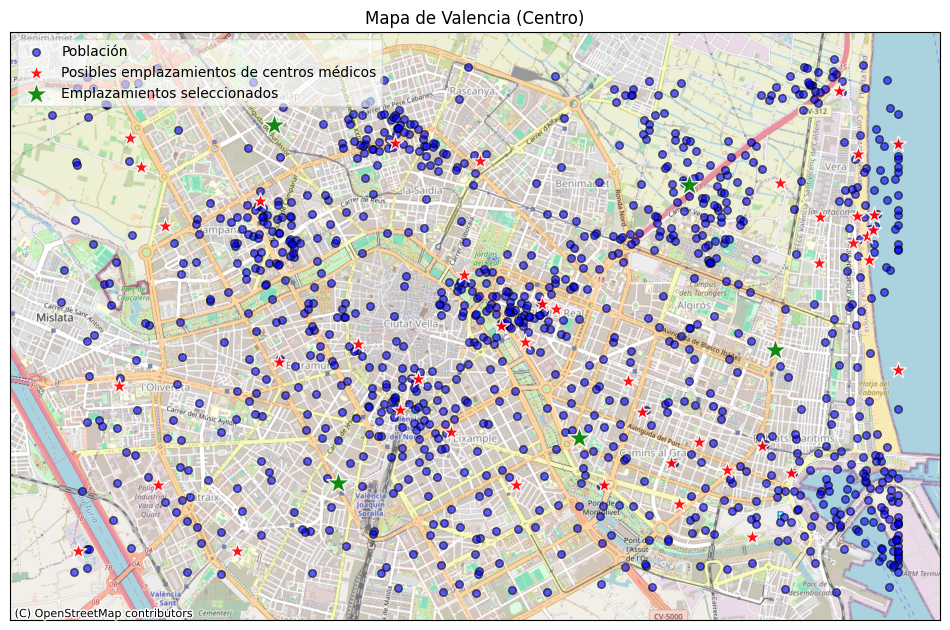
\includegraphics[width=\textwidth]{images/equilibrada.png}
        \caption{Solución encontrada por el algoritmo equilibrando la carga de los centros.}
        \label{fig:equilibrada}
    \end{subfigure}
    
    \caption{Ejemplo del problema de localización: (a) población y sitios potenciales, y (b-d) tres posibles soluciones con distintos niveles de eficacia.}
    \label{fig:casos_ejemplo}
\end{figure}

El objetivo será encontrar todas las soluciones al Frente de Pareto, no únicamente las extremas tomando como referencia una única
función objetivo. La manera de llevar esto a cabo será por medio de metaheurísticos, al ser un problema de combinatoria NP-difícil (demostrado en \cite{k-balanced_1} que el problema es NP-completo). Para ello, 
se va a definir el modelo matemático.

\section{Modelo Matemático}
Sean $N=\{1, 2, \dots, n\}$ el conjunto de \textbf{puntos de demanda} y $M=\{1, 2, \dots, m\}$ el conjunto de ubicaciones para las \textbf{potenciales instalaciones}.

Se define $d_{ij}$ como la distancia entre el punto de demanda $i \in N$ y la ubicación $j \in M$.\\
El conjunto de variables de decisión será $X$. Cada una de las variables $x_j \in X$ toma valores en $\{0,1\}$, siendo 1 si la ubicación $j \in M$ se selecciona y 0 en caso contrario. Como debe haber $k$ ubicaciones seleccionadas:
\begin{equation}
    \sum_{j \in M} x_j = k
\end{equation}

Se asume que cada punto de demanda es atendido por la instalación más cercana dentro del conjunto de localizaciones $M$. En base a esto, se define $n_j$ como la cantidad de puntos de demanda asignados a la instalación $j \in M$.

El problema da lugar a las siguientes tres funciones objetivo:

\begin{equation}
    \text{Minimizar} \quad f_1(X) = \max_{i \in N} \min_{j \in M} d_{ij}
    \label{eq:f1}
\end{equation}
Esta función, propia de los problemas \textit{k-centro}, busca minimizar la \textbf{distancia máxima} que debe recorrer cualquier cliente hasta su instalación asignada. El objetivo es lograr la mejor cobertura posible, evitando que algún punto de demanda quede excesivamente lejos.

\begin{equation}
    \text{Minimizar} \quad f_2(X) = \max_{j \in M} n_j
    \label{eq:f2}
\end{equation}
El objetivo de $f_2$ es minimizar la carga de trabajo de la instalación más congestionada. 

\begin{equation}
    \text{Minimizar} \quad f_3(X) = \max_{\substack{j, j' \in M \\ j \neq j'}} |n_j - n_{j'}|
    \label{eq:f3}
\end{equation}
La función $f_3$ minimiza la diferencia entre la instalación con más carga y la que tiene menos. Es el objetivo más estricto en términos de \textbf{equidad operativa}, ya que busca que todas las instalaciones tengan una carga de trabajo lo más homogénea posible.

Recopilando lo visto hasta ahora, se deducen las siguientes características clave del problema:

\begin{itemize}
    \item \textbf{Optimización no lineal}: Las funciones objetivo son no lineales, ya que contienen operadores como $\max$, $\min$ y valor absoluto.
    
    \item \textbf{Optimización discreta}: El dominio de la solución es discreto, pues se debe elegir un subconjunto de un conjunto finito de ubicaciones.
    
    \item \textbf{Problema combinatorio NP-difícil}: El problema consiste en encontrar el mejor subconjunto de $k$ elementos de un total de $m$. El número de soluciones posibles es $\binom{m}{k}$ (ver en \ref{def:combinatorio}).
    
    \item \textbf{Problema multiobjetivo}: Se desean optimizar simultáneamente tres funciones objetivo.
\end{itemize}

Tomando en cuenta esto, se va a proponer el algoritmo metaheurístico para resolver el problema.


\chapter{Resolución del problema}
Para resolver el \textbf{Problema Multiobjetivo de Localización de k-Centros Balanceado}, se va a utilizar un algoritmo \textit{GRASP} (\textit{Greedy Randomized Adaptive Search Procedure}).
El algoritmo constará de dos partes principales, una primera de generación de solución inicial y una segunda en la que se mejorará mediante búsqueda local aplicada a esta solución.

El funcionamiento de la búsqueda local problemas monoobjetivo es mucho más sencillo de definir, principalmente se mejora en base a una única función objetivo, y nunca al realizar una búsqueda local se puede dar el caso de que la solución empeore. En Multiobjetivo es más delicado,
se tiene que tener en cuenta que la mejora de una única de las funciones objetivo puede que no ayude a aproximar ninguna solución.

Para ello, se ha diseñado una búsqueda local que tiene en cuenta las tres funciones objetivo, y otras tres búsquedas locales direccionales para encontrar soluciones en zonas más prometedoras.

\section{¿Por qué el GRASP?}
Se ha elegido \textit{GRASP} como base metodológica por varias razones que lo hacen especialmente adecuado para el Problema Multiobjetivo de Localización de k-Centros Balanceado:
\begin{itemize}
    \item \textbf{Flexibilidad de adaptación}: El \textit{GRASP} es un método relativamente sencillo de codificar, pero con una ampla variedad de posibilidades
    a la hora de ajustar tanto la fase de construcción como de mejora, para adaptarse a casi cualquier escenario posible. 
    \item \textbf{Buen desempeño}: A diferencia de otros algoritmos como la Búsqueda Tabú o los Genéticos, que requieren de tiempos más prolongados de ejecución para encontrar buenas soluciones,
    \textit{GRASP} obtiene buenos resultados sin requerir de muchas iteraciones para llegar a ellos.
    \item \textbf{Adecuación a problemas combinatorios}: El método resulta especialmente apropiado para resolver problemas combinatorios, ya que la definición de movimientos de mejora en la búsqueda local es intuitiva y directa.
    Esto permite explorar el espacio de soluciones de manera eficaz y con un coste computacional relativamente bajo.
    \item \textbf{Madurez y respaldo en la literatura}: \textit{GRASP} ha sido desarrollado y probado en una amplia gama de problemas, incluyendo problemas de optimización multiobjetivo. Algunos ejemplos son \cite{grasp_1}, \cite{grasp_3} y \cite{grasp_2}. 
\end{itemize}

\section{Estado del arte}

\subsection{Artículo 1}
El primer trabajo relevante en la literatura es el de \cite{k-balanced_1}, en el cual se propone formalmente el problema de localización multiobjetivo de $k$-centros balanceado y se presenta una primera estrategia de resolución mediante el algoritmo \textit{MOAkBCL}.
Este enfoque parte de la triangulación de Delaunay \citep{delaunay} y construye soluciones mediante intercambios locales, siguiendo una lógica muy cercana al algoritmo evolutivo \textit{NSGA-II}.

El primer paso del algoritmo consiste en emplear esta triangulación para definir la ``vecindad'' entre instalaciones. Dos instalaciones se consideran vecinas de una tercera si, 
dentro del área que delimita la circunferencia circunscrita al triángulo formado por las tres, no se encuentra ninguna otra instalación. 

Una vez obtenida una solución inicial, la manera de encontrar nuevas soluciones es intercambiar centros seleccionados por alguno de sus vecinos. El procedimiento general del algoritmo es el siguiente:

\begin{enumerate}
    \item Se inicializan los parámetros principales, incluyendo el tamaño de la población y el número máximo de iteraciones. A continuación, se genera una población inicial de soluciones aleatorias.
    \item Cada solución es evaluada de acuerdo con las tres funciones objetivo.
    \item A partir de la población actual de soluciones, se generan nuevas mediante intercambios de centros seleccionados por otros que pertenezcan a su vecindad. Entre las soluciones originales y las nuevas se construyen frentes
    de Pareto: el primero con las soluciones no dominadas, el segundo con aquellas dominadas únicamente por el frente 1, y así sucesivamente hasta clasificar todas. 
    \item Para filtrar las soluciones, se tiene en cuenta tanto que pertenezcan al frente más bajo posible como a que estén lo más alejadas entre sí, con el fin de preservar la diversidad. 
    \item Este procedimiento se repite hasta alcanzar el número máximo de iteraciones,  extrayéndose finalmente el Frente de Pareto en la última iteración.
\end{enumerate}
Gracias a esta forma de buscar nuevas soluciones aprovechando la geometría de las instalaciones, el algoritmo se demuestra más eficiente que el \textit{NSGA-II}, el utilizado como 
referencia para comparar los resultados. 

Aparte del método para resolver el problema, se demuestra que efectivamente el problema es NP-completo (si es NP-completo, es NP-difícil), e incluso que encontrar una única
solución del Frente de Pareto es NP-Completo.

\subsection{Artículo 2}
El segundo trabajo es el de \cite{k-Balanced_2}, en el que se plantea una alternativa al enfoque evolutivo anterior. En este caso, se propone un método híbrido basado en la metaheurística \textit{GRASP}, complementado con Oscilación Estratégica y \textit{Path Relinking}. El objetivo principal es mejorar la capacidad exploratoria del algoritmo, permitiendo visitar tanto soluciones factibles como no factibles para, posteriormente, transformarlas en configuraciones válidas de alta calidad.

El procedimiento comienza con la generación de una población inicial de soluciones mediante un esquema greedy randomizado. Este mecanismo permite construir soluciones iniciales de buena calidad, cada una definida por la selección de $k$ centros. Posteriormente, se aplica una fase de búsqueda local propia del \textit{GRASP}, basada en intercambiar elementos de la solución por otros que no forman parte de ella, siempre que el nuevo candidato no resulte dominado por el conjunto de soluciones actuales.

A partir de esta población inicial, se incorpora la estrategia de Oscilación Estratégica, cuyo propósito es diversificar la búsqueda explorando regiones más amplias del espacio de soluciones. Para ello, el algoritmo altera temporalmente la factibilidad de las soluciones: por un lado, añadiendo elementos hasta generar configuraciones sobredimensionadas; por otro, reduciendo el número de elementos por debajo del umbral permitido.
Este proceso iterativo favorece la identificación de regiones prometedoras que, de otro modo, permanecerían inexploradas.

Finalmente, el enfoque introduce el uso innovador de \emph{Path Relinking} como mecanismo de reparación. A partir de soluciones no factibles —ya sea con exceso o con déficit de elementos—, se construyen trayectorias que exploran soluciones intermedias, priorizando aquellas que comparten características comunes con ambas configuraciones iniciales. De este modo, se obtienen nuevas soluciones factibles de alta calidad.

Cabe resaltar que este es el primer algoritmo en utilizar \emph{Path Relinking} para la reparación de soluciones generadas por Oscilación Estratégica, lo cual constituye una aportación metodológica relevante. Los resultados experimentales demuestran que el enfoque propuesto supera a algoritmos de referencia ampliamente utilizados, como \textit{NSGA-II}, \textit{MOEA/D} y \textit{SPEA2}, tanto en eficiencia como en calidad de las soluciones obtenidas.

\section{Algoritmo Propuesto}
El funcionamiento general de implementación de un algoritmo \textit{GRASP} es el siguiente:

\begin{algorithm}[H]
\caption{Algoritmo GRASP}
\begin{algorithmic}[1]
\Statex \textbf{Definiciones:}
\Statex \hspace{1em} \texttt{MAX\_ITS}: número máximo de iteraciones
\Statex \hspace{1em} \texttt{SolMejor}: mejor solución encontrada
\Statex \hspace{1em} \texttt{ValorMejor}: valor de la mejor solución

\Statex

\State Inicializar \texttt{SolMejor} $\gets \emptyset$, \texttt{ValorMejor} $\gets -\infty$
\For{$\texttt{its} = 1$ \textbf{hasta} \texttt{MAX\_ITS}}
    \Statex \textbf{// Fase de construcción}
    \State $X^{(0)}\gets$ \texttt{ConstruccionGreedyRandomizada}($\alpha$)
    
    \Statex \textbf{// Fase de búsqueda local}
    \State $X^{(1)}\gets$ \texttt{BusquedaLocal}($X^{(0)}$)

    \If{\texttt{Evaluar}($X^{(1)}$) $>$ \texttt{ValorMejor}}
        \State \texttt{SolMejor} $\gets X^{(1)}$
        \State \texttt{ValorMejor} $\gets$ \texttt{Evaluar}($X^{(1)}$)
    \EndIf
\EndFor
\State \Return \texttt{SolMejor}


\end{algorithmic}
\end{algorithm}

Este esquema hará más sencillo entender las partes en las que se ha dividido el algoritmo \textit{GRASP} con \textit{Multi-Armed Bandits} propuesto para este trabajo.

Antes de empezar a definirlo, en el desarrollo de las funciones de evaluación tanto de $f_2$ como de $f_3$ hay que tener en cuenta la posibilidad de empates. Esto podría influir en la obtención de unas u otras soluciones para el Frente de Pareto. 
En tales casos, podría ser factible redistribuir los empates hacia emplazamientos seleccionados con menor carga de demanda, con el fin de obtener mejoras adicionales en dichas funciones objetivo.  

No obstante, esta estrategia no se ha implementado en el algoritmo actual, ya que en el presente estudio no se han observado instancias en las que resultase necesaria. Sin embargo, en uno de los trabajos previos revisados se identificaron situaciones en las que el redondeo de distancias podía generar soluciones degradadas (véase \ref{sec:articulo2}).  

\subsection{Fase de Construcción: Algoritmo Greedy Randomizado}
La construcción de la solución inicial constituye el primer paso del procedimiento. El objetivo es generar una solución de calidad aceptable en un tiempo reducido, incorporando además un componente de aleatoriedad que favorezca la exploración de distintas regiones del espacio de búsqueda.  

El algoritmo Greedy Randomizado sigue la siguiente secuencia:  

\begin{itemize}
    \item \textbf{Inicialización:} Se selecciona de manera aleatoria un centro de suministro inicial entre los $m$ disponibles.
    \item \textbf{Construcción iterativa:} Mientras no se hayan seleccionado las $k$ instalaciones requeridas:
    \begin{itemize}
        \item Se evalúan los centros candidatos no seleccionados, calculando el valor de la función objetivo $f_1$ (véase \ref{eq:f1}) suponiendo la incorporación de cada uno de ellos. Se utiliza exclusivamente $f_1$ con el fin de evitar una complejidad excesiva en esta fase y porque es la función objetivo que puede generar soluciones más realistas y balanceadas.
        \item \textbf{Lista Restringida de Candidatos (RCL):} En lugar de escoger siempre el mejor candidato, se construye una lista con aquellos cuyos valores se encuentran próximos dicho candidato. El parámetro $\alpha$ regula el nivel de aleatoriedad:
        \begin{itemize}
            \item Si $\alpha = 0$, la RCL contiene únicamente el mejor candidato (máxima voracidad).
            \item Si $\alpha = 1$, la RCL incluye a todos los candidatos (máxima aleatoriedad).
        \end{itemize}
        Por último se escoge al azar uno de los centros de la RCL y se incorpora a la solución.
    \end{itemize}
\end{itemize}

Este procedimiento semi-aleatorio garantiza que cada ejecución del \textit{GRASP} explore una variedad más amplia de soluciones iniciales, equilibrando exploración y explotación: se preserva la diversidad sin sacrificar la calidad de las soluciones generadas. La influencia del parámetro $\alpha$ en la eficacia de esta fase se analizará más adelante en la Figura~\ref{fig:alpha}.

\subsection{Fase de Búsqueda Local}
Una vez construida la solución inicial, se procede a su mejora mediante un proceso de búsqueda local basado en intercambios. El procedimiento consiste en ir seleccionando, por orden de aparición en la solución, cada elemento e ir intercambiándolo por cada uno de los que no aparecen en ella (igualmente, por orden de aparición en los datos). Para cada intercambio se evalúan las tres funciones objetivo; si la nueva solución domina a la solución actual, se adopta el cambio y la nueva solución pasa a ser la actual. No se busca el intercambio globalmente óptimo, sino el primero que cumpla el criterio de dominancia, es decir, el primer elemento que, al meterlo en la solución la mejore, entra de reemplazo. 

El proceso se repite hasta recorrer en un ciclo completo los $k$ elementos de la solución sin obtener ninguna mejora.

Tras cada búsqueda local, la solución resultante se compara con el Frente de Pareto actual. Si la solución está dominada, se descarta. En caso contrario, se eliminan las soluciones del frente que resulten dominadas por la nueva, y finalmente esta se incorpora al conjunto de soluciones. De este modo, únicamente se conservan las soluciones pertenecientes al Frente de Pareto vigente.

Posteriormente, se ejecuta una búsqueda local direccional con el propósito de diversificar el proceso hacia regiones menos exploradas del espacio de soluciones, en las que es posible identificar nuevos óptimos.  

Las búsquedas direccionales consideradas son:  

\begin{itemize}
    \item \textbf{Búsqueda local respecto a $f_1$ \ref{eq:f1}:} Minimiza la distancia máxima entre los centros seleccionados y los elementos de la población.
    \item \textbf{Búsqueda local respecto a $f_2$ \ref{eq:f2}:} Reduce la carga máxima de clientes asignados a un centro.
    \item \textbf{Búsqueda local respecto a $f_3$ \ref{eq:f3}:} Disminuye la diferencia de cargas entre el centro más demandado y el menos utilizado.
\end{itemize}

Estas búsquedas se implementan de manera análoga a la búsqueda local general, pero considerando únicamente la función objetivo correspondiente a la dirección elegida. En la siguiente subsección se detallará el mecanismo empleado para seleccionar qué búsqueda aplicar y el número máximo de iteraciones permitidas para cada una.

\subsection{Aprendizaje Reforzado: \textit{Multi-Armed Bandits}}
Como se ha mencionado previamente, el algoritmo necesita un mecanismo para decidir en qué dirección y con qué intensidad debe desplazarse tras obtener la primera solución mediante búsqueda local. El modelo de \textit{Multi-Armed Bandit} se utilizará con esta función, determinando tanto la dirección de la búsqueda local como la magnitud del esfuerzo de mejora.

El \textit{MAB} utilizado está compuesto por los siguientes elementos:

\begin{itemize}
    \item \textbf{Agente:} El propio algoritmo, que ``aprende'' progresivamente a seleccionar las mejores direcciones en las que buscar las nuevas soluciones.
    
    \item \textbf{Entorno:} El espacio de soluciones factibles.
    
    \item \textbf{Tiempo:} Cada una de las búsquedas locales direccionales realizadas durante la ejecución del algoritmo.
    
    \item \textbf{Estado ($S$):} Se define a partir de la información disponible sobre la solución actual y las soluciones del Frente de Pareto. Concretamente, se extrae un \textbf{contexto ($C$)} representado como una tupla de tres componentes $(C^1, C^2, C^3)$, donde cada componente indica la distancia necesaria para que la solución actual deje de ser dominada, es decir, cuánto debería mejorar en cada uno de los objetivos.
    
    Por ejemplo, un contexto $(0, 0, 0)$ indica que la solución ya pertenece al Frente de Pareto. En cambio, un contexto $(30, 15, 10)$ sugiere que la solución debería mejorar 30 unidades en $f_1$, o 15 en $f_2$, o 10 en $f_3$ para ser no dominada.

    \item \textbf{Acción:} Las acciones posibles corresponden a los ``brazos'' del \textit{MAB}. Cada brazo representa una combinación entre:
    \begin{itemize}
        \item La dirección de la búsqueda local ($f_1$, $f_2$ o $f_3$).
        \item El número máximo de mejoras consecutivas permitidas ($1, 2, \dots, k$).
    \end{itemize}

    La selección de la acción se realiza con el siguiente criterio:
    \begin{itemize}
        \item Con probabilidad $\beta$, se elige una acción aleatoria (exploración).
        \item Con probabilidad $1 - \beta$, se selecciona una acción de forma probabilística, ponderada según su recompensa esperada (explotación). Aunque las acciones con mayor recompensa esperada tienen más probabilidad de ser elegidas, no se garantiza su selección determinista.
    \end{itemize}

    Para evitar que acciones con recompensas extremas dominen completamente la selección o sean injustamente descartadas, se aplica la función \textit{softmax} para normalizar los valores esperados:
    \begin{equation}
        \sigma(z)_i = \frac{e^{z_i - \max(z)}}{\sum_{j=1}^{K} e^{z_j - \max(z)}}
    \end{equation}

    \item \textbf{Recompensa:} Tras ejecutar una acción, se mide su efectividad evaluando el contexto antes y después de la búsqueda local. La recompensa se define de la siguiente forma:
    \begin{itemize}
        \item \textbf{Caso 1:} Se asigna una recompensa de $5$ si la acción genera una solución nueva no dominada (es decir, una mejora real en el frente).
        \item \textbf{Caso 2:} Se asigna una recompensa de $-1$ si no se obtiene ninguna solución nueva no dominada.
    \end{itemize}

    Finalmente, la matriz de pesos del \textit{MAB} se actualiza en función de la recompensa obtenida, reforzando las acciones que han resultado efectivas en contextos similares.
\end{itemize}

\newpage

\section{Implementación}

\begin{algorithm}[H]
\caption{Algoritmo \textit{GRASP-MAB}}
\begin{algorithmic}[1]
    \Statex \textbf{Definiciones:}
    \Statex \hspace{1em} \texttt{MAX\_ITS}: número máximo de iteraciones
    \Statex \hspace{1em} \texttt{W}: pesos del MAB
    \Statex \hspace{1em} \texttt{F}: frente de soluciones
    \Statex \hspace{1em} $X^{(0)}$: solución inicial
    \Statex \hspace{1em} $X^{(i)}$: solución modificada en la fase $i$
    \Statex \hspace{1em} \texttt{C}: contexto extraído de la solución y el frente
    \Statex \hspace{1em} \texttt{R}: recompensa asociada a la mejora de la solución

    \Statex

    \State Inicializar \texttt{W}, \texttt{F} $\gets \emptyset$
    \For{$\texttt{its} = 1$ \textbf{hasta} \texttt{MAX\_ITS}}
        \Statex \textbf{// Construcción y búsqueda local inicial}
        \State $X^{(0)}\gets$ \texttt{ConstruccionGreedyRandomizada}($\alpha$) // Se construye la solución inicial
        \State $X^{(1)}\gets$ \texttt{BusquedaLocal}($X^{(0)}$)
        \State \texttt{ActualizarFrente}($X^{(1)}$, F)
        \State \texttt{mejora} $\gets$ \texttt{true} // Se inicializa la variable mejora como true para que siempre haga una búsqueda local direccional.
        
        \While{\texttt{mejora}}
            \Statex \textbf{// Extracción de contexto y selección de brazo}
            \State \texttt{C} $\gets$ \texttt{ExtraerContexto}($X^{(1)}$, F)
            \State \texttt{brazo} $\gets$ \texttt{SeleccionarBrazoMAB}(W, C)
            
            \Statex \textbf{// Búsqueda local dirigida}
            \State $X^{(2)}\gets$ \texttt{BusquedaLocalDireccional}($X^{(1)}$, brazo)
            \State $X^{(3)}\gets$ \texttt{BusquedaLocal}($X^{(2)}$)
            
            \If{$X^{(3)}$ mejora el frente}
                \State \texttt{$X^{(1)}$} $\gets$ $X^{(3)}$
                \State \texttt{ActualizarFrente}($X^{(3)}$, F)
                \State \texttt{mejora} $\gets$ \texttt{true}
                \State \texttt{R} $\gets 5$
            \Else
                \State \texttt{mejora} $\gets$ \texttt{false}
                \State \texttt{R} $\gets -1$
            \EndIf

            \State \texttt{ActualizarPesosMAB}(W, brazo, R)
        \EndWhile
    \EndFor
    \State \Return \texttt{F}
\end{algorithmic}
\end{algorithm}

En el pseudocódigo, se inicializan las variables en la línea 1, en las líneas 2 y 3 se encuentra la fase de construcción, la línea 4
es la búsqueda local y el bucle que inicia en la línea 7 y termina en la 20 el \textit{Multi-Armed Bandit} itera seleccionando una búsqueda local direccional
y mejorando la solución $X^{(2)}$ con otra búsqueda local. Esta última parte se repite mientras se sigan encontrando soluciones no dominadas para el Frente de Pareto.


Con esta representación se puede ver de una manera más sencilla el funcionamiento del algoritmo implementado en Python. Tanto los datos, Frentes de Pareto encontrados, soluciones, como el código, se encuentran en el repositorio de GitHub: \url{https://github.com/Manumrm8/TFM_optimization.git}.

Para agilizar el algoritmo, aparte de reducir los tiempos de ejecución todo lo posible simplificando código, se ha optado por utilizar la librería ``multiprocessing'' para paralelizarlo.
El aumento de rendimiento dependerá del procesador utilizado para ejecutar el código. A más núcleos mayor mejora.

Al haberse paralelizado, se ha de tener en cuenta que no se puede, sin reducir en gran medida la velocidad del algoritmo, hacer que el conjunto de instancias paralelizadas compartan
el mismo Frente de Pareto encontrado o los mismos pesos del \textit{MAB}. Por tanto, cada instancia tendrá tanto su archivo de pesos como de soluciones. Al terminar las ejecuciones, se combinan los Frentes de Pareto de 
todas las ejecuciones y se obtiene el Frente de Pareto común.

Al final, comparando los resultados tanto de ejecutar las instancias en paralelo como en serie, no difieren significativamente en el rendimiento, que no en tiempo, con lo que paralelizar tanto soluciones como pesos no empeora 
el algoritmo.

\chapter{Experimentación y Resultados}

Para evaluar el rendimiento del algoritmo, se han utilizado dos instancias ya trabajadas tanto en el artículo \cite{k-balanced_1} como en el \cite{k-Balanced_2}. 

Ambas constan de los mismos 1000 puntos de demanda y las mismas 50 potenciales instalaciones, distribuidas en una cuadrícula de 1500 unidades de largo por 1000 de ancho.
La diferencia radica en que en la primera, \textit{WorkSpace 1000\_50\_5}, $k=5$, por lo que será más asequible encontrar soluciones al rondar las combinaciones los 2 millones, mientras que en la segunda, \textit{WorkSpace 1000\_50\_10}, $k=10$, el problema pasa a ser mucho más complejo, rondando las diez mil millones de combinaciones.

La primera se ha utilizado tanto en los ejemplos mostrados en la Figura~\ref{fig:centros_medicos} como para ajustar los parámetros del algoritmo. Finalmente, en el apartado de comparativa
se expondrá el rendimiento del algoritmo en ambas instancias.

\section{Fine tuning}

Primero, se van a evaluar las tres variables a ajustar:
\begin{itemize}
    \item \textbf{Alpha ($\alpha$)}: Durante la inicialización de las soluciones greedy, en cada paso se incorpora un elemento $x_i$ a la solución. El parámetro $1-\alpha$ determina el porcentaje de los mejores candidatos $x_i \in X, \; x_i \neq 1$ entre los cuales se selecciona.  
Si $\alpha = 1$, siempre se elige el mejor candidato; si $\alpha = 0$, la elección es completamente aleatoria. En términos generales, el procedimiento consiste en escoger aleatoriamente un $x_i$ dentro del conjunto de los $(1-\alpha)$ mejores candidatos.
    \item \textbf{Beta ($\beta$)}: El rendimiento del \textit{MAB} depende en gran medida del equilibrio entre exploración y explotación. El parámetro $\beta$ regula, durante la selección de la búsqueda local en el \textit{GRASP}, qué proporción de elecciones se realiza de manera aleatoria y cuál de forma probabilística ponderada según los pesos del \textit{MAB}.  
Si $\beta = 0$, la selección es siempre probabilística y ponderada; si $\beta = 1$, la elección es completamente aleatoria.
    \item \textbf{Learning Rate ($lr$)}: Tasa de aprendizaje del \textit{MAB}. Define cuánto influye la recompensa y el contexto en la actualización de los pesos. 
Un valor pequeño de $lr$ produce actualizaciones más suaves y estables, mientras que un valor grande genera cambios más rápidos y pronunciados.
\end{itemize}

Se empieza ajustando el parámetro $lr$ del \textit{MAB}, ya que es necesario para que el aprendizaje reforzado sea efectivo. Un $lr$ muy bajo hace que los pesos no se modifiquen, y todas las acciones tengan probabilidades parecidas, mientras uno alto hace que las acciones estén muy descompensadas y no reflejar la realidad del valor esperado de la acción.

El valor final escogido ha sido $lr=0.1$, utilizando valores entre 0.01 y 2.

Una vez ajustado el learning rate, se busca el $\beta$, tomando candidatos en el rango $[0,1]$ con los valores $0, 0.1, 0.2, \dots, 0.9, 1$.  
Para cada valor de $\beta$, el algoritmo se ejecuta en paralelo en 20 instancias independientes, cada una de ellas corriendo con una duración total de 100 iteraciones. 
En total, esto equivale a 220 ejecuciones simultáneas, lo que permite observar la evolución del algoritmo y disponer de un espacio muestral suficiente para comparar su desempeño bajo distintos valores de $\beta$.

Los resultados se representarán mediante \textit{diagramas de caja}, los cuales permiten visualizar de manera resumida la distribución de los datos. 
En primer lugar, una línea negra dentro de la caja marca la posición de la \textbf{mediana} (\ref{def:mediana}), que indica el valor central de los datos. 
La propia caja encierra el 50\% de las observaciones, delimitada por el \textbf{primer cuartil} (\ref{def:cuartil}), en su borde inferior, y el \textbf{tercer cuartil}, en su borde superior. 
A continuación, los \textbf{bigotes} se extienden hasta los valores que se encuentran a una distancia máxima de 1.5 veces el \textbf{rango intercuartílico} (\ref{def:iqr}) a partir de los cuartiles. 
Finalmente, los \textbf{valores atípicos}, es decir, aquellos que sobrepasan este límite, se representan de manera individual mediante puntos vacíos.
\begin{figure}[htbp!]
    \centering
    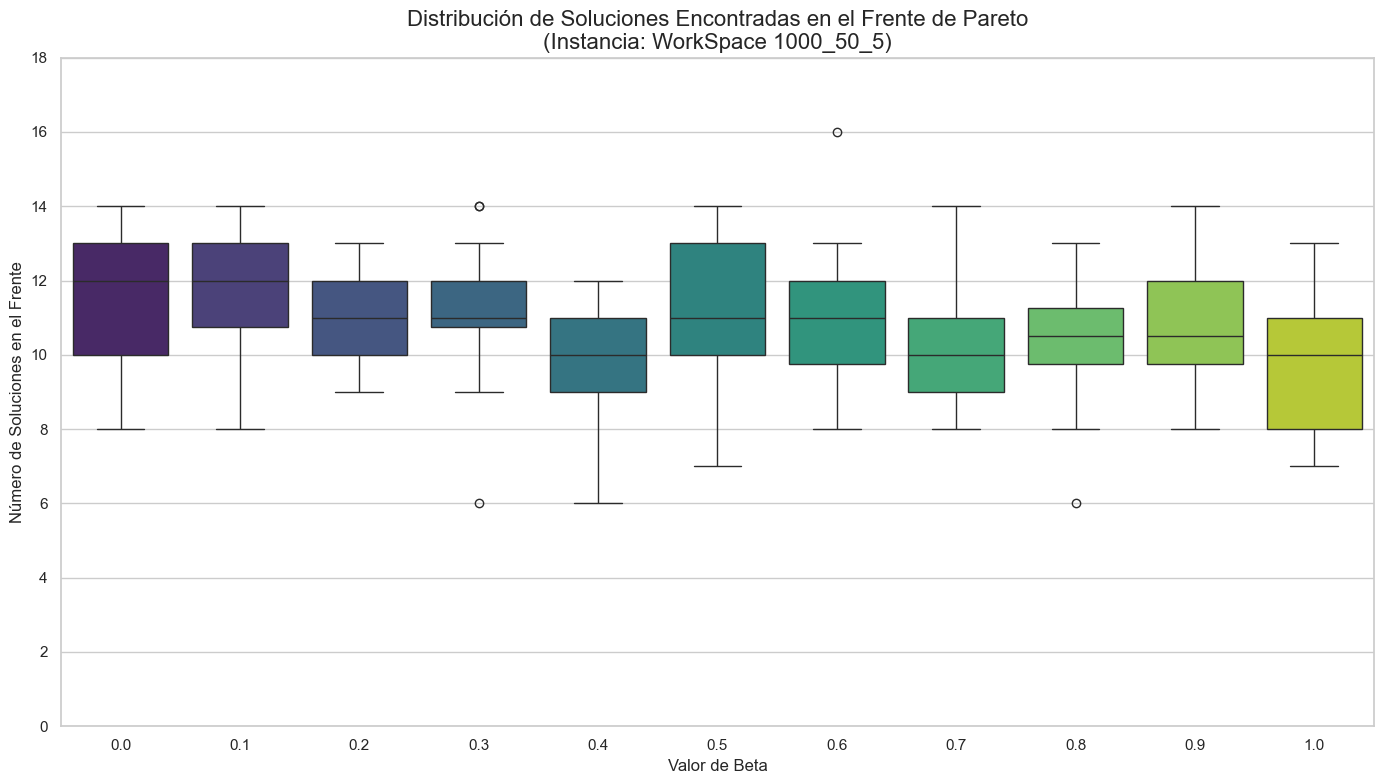
\includegraphics[width=0.8\linewidth]{images_finetuning/beta_20_100.png}
    \caption{Diagrama de cajas con las soluciones en el Frente de Pareto agrupadas por $\beta$.}
    \label{fig:beta}
\end{figure}

En la Figura~\ref{fig:beta} se puede ver que utilizar aprendizaje reforzado se llega a aumentar en hasta un 20 \% el rendimiento del algoritmo. Con $\beta=1$ los resultados rondan en torno a una mediana de $10$ soluciones mientras que valores cercanos a $0$ rondan las $12$ soluciones. Por tanto, se ha decidido tomar el $\beta=0.1$

Para terminar, se ajusta el parámetro $\alpha$ en el rango $[0,1]$, dividido en los mismos 11 valores equiespaciados: $0, 0.1, 0.2, \dots, 0.9, 1$.  
Para cada valor de $\alpha$, el algoritmo también se ejecuta en paralelo en 20 instancias independientes, cada una de ellas corriendo con una duración total de 100 iteraciones.


\begin{figure}[htbp!]
    \centering
    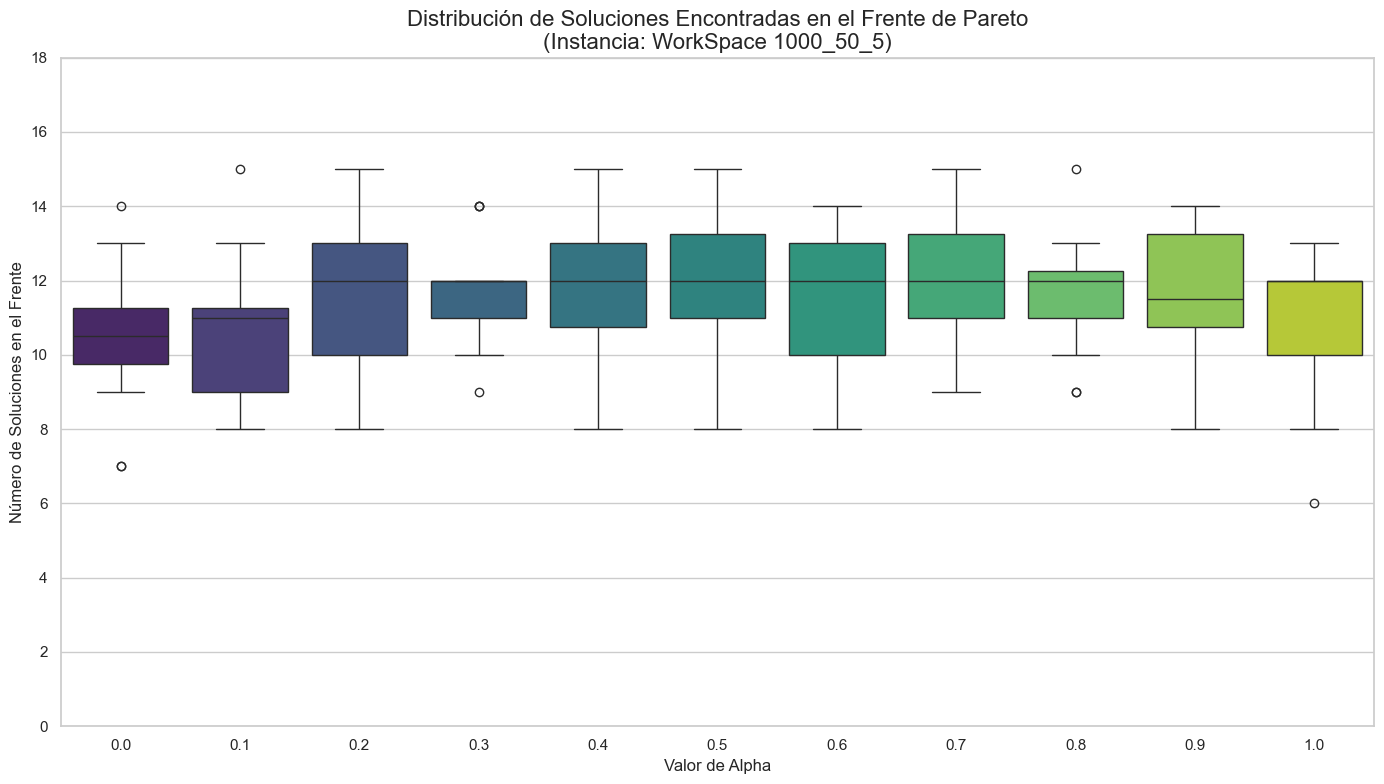
\includegraphics[width=0.8\linewidth]{images_finetuning/alpha_20_100}
    \caption{Diagrama de cajas con las soluciones en el Frente de Pareto agrupadas por $\alpha$.}
    \label{fig:alpha}
\end{figure}

Se puede ver en la Figura~\ref{fig:alpha} que lo ideal es tomar valores de alpha entre $0.2$ y $0.8$, sin una diferencia clara entre los mismos. Por tomar arbitrariamente alguno de los valores, se decide por $\alpha=0.3$.

\section{Resultados de los artículos}

\subsection{Primera vista a los resultados previos}
\label{sec:articulo2}
Tomando como referencia las soluciones reportadas en el artículo \cite{k-Balanced_2}, se realizó una comparación para verificar si el método \textit{GRASP} desarrollado en este TFM alcanzaba los mismos resultados. De este análisis se observó que, en algunos casos, se obtuvieron soluciones superiores a las allí presentadas, mientras que en otros los resultados fueron menos favorables.
Sin embargo, dado que en dicho artículo no se proporcionan los componentes exactos de cada solución, una evaluación directa no es posible. 
Además, los valores de la función objetivo $f_1$ aparecen truncados a nivel decimal, lo que sugiere que las distancias fueron redondeadas.

Si en este trabajo se aplican también redondeos sobre las soluciones, se constata que se alcanzan Frentes de Pareto muy similares, aunque con ligeras diferencias en $f_2$ y $f_3$. Asumiendo que las premisas anteriores son correctas, cabe señalar que en algunos casos no se habría contemplado el efecto de los empates generados por el redondeo de las distancias. Para ilustrar esto, consideremos el siguiente ejemplo encontrado:

Los posibles emplazamientos se numeran del 0 al 49, al igual que cada punto de demanda se numera desde el 0 al 999. Una de las soluciones reportadas en el artículo es (suponiendo que sea la misma que en una búsqueda exhaustiva del Frente de Pareto) $X_1 = [13, 20, 23, 29, 49]$, cuyos valores son $f_1(X_1) = 415$, $f_2(X_1) = 232$ y $f_3(X_1) = 128$. En cambio, al evaluar esta misma solución en el presente TFM se obtuvieron $f_1'(X_1) = 415$, $f_2'(X_1) = 233$ y $f_3'(X_1) = 129$.
El análisis muestra que, tras redondear las distancias y revisar la saturación de las instalaciones, la instalación 20 recibió $233$ elementos. Al analizar los empates, se observó que los puntos de demanda 435 y 827 estaban equidistantes entre las instalaciones 20 y 13, la cual contaba con $228$ elementos asignados.

Se puede entonces suponer que en los resultados del artículo se habría asignado uno de estos puntos de demanda a la instalación 20 y el otro a la 13, obteniendo así los valores publicados. Sin embargo, también podría plantearse que, bajo un redondeo estricto, la solución no sería óptima.
De hecho, si ambos puntos de demanda se asignan a la instalación 13, se obtendría $f_2 = 231$ y $f_3 = 127$.

En conclusión, este análisis evidencia que la manera de resolver los empates al asignar los puntos de demanda a las instalaciones más cercanas puede resultar determinante en la evaluación de las soluciones.

\subsection{Comparativa}

Antes de presentar las tablas, se ajustó el número de ejecuciones de los algoritmos para los tiempos coincidan con los contenidos en el artículo \cite{k-balanced_1}, con el fin de realizar una comparativa lo más justa posible. Para la primera instancia (\ref{tab:ws1000_50_5}) se correrán a 220 iteraciones, mientras que para la segunda (\ref{tab:ws1000_50_10}) a 176.

Como se mencionó en el resumen, por un lado, los algoritmos \textit{GRASP} estarán peor optimizados al ejecutarse en 
Python en comparación con las implementaciones previas; sin embargo, el procesamiento será más rápido al haber utilizado una memoria RAM y un procesador con más núcleos en sus ejecuciones. Por este motivo, las comparaciones se presentan con una posible desventaja de los algoritmos \textit{GRASP} con respecto a las implementaciones previas.

Así mismo, la comparación se va a limitar al primer artículo, dado a que solo se han realizaron pruebas con la instancia \textit{WorkSpace 1000\_50\_5} y con la \textit{WorkSpace 1000\_50\_10}, mientras que los resultados del segundo artículo no están desglosados 
por instancia sino promediados entre todas ellas, lo que impide una comparación directa por caso.

Para disponer de un ``Frente de Pareto exacto'' de referencia en la Tabla~\ref{tab:ws1000_50_5}, se ha extraído iterando sobre el conjunto completo de combinaciones posibles.
Aunque el problema es NP-difícil, para instancias pequeñas es posible recorrer todas las combinaciones en tiempos razonables. En este caso, aproximadamente 30 min para comprobar las más de 2 millones de combinaciones. 

Esto no se puede decir de la segunda instancia en \ref{tab:ws1000_50_10}, al multiplicar por 10,000 el número de combinaciones, lo que hace inviable este método. Por ello, como referencia tanto para los resultados del \textit{GRASP} como del \textit{MAB-GRASP},
se ha corrido el algoritmo \textit{MAB-GRASP} durante 2 horas, y el Frente de Pareto encontrado es el que se ha tomado como aproximación del Frente de Pareto exacto.

Para comparar se utilizará la métrica de coverage, formulada:
$$coverage(F',F) = \frac{\left| \{\, f' \in F' \;\mid\; \exists f \in F : f \preceq f' \,\} \right|}{|F'|}.$$
Es decir, la cantidad de soluciones encontradas no dominadas en $F'$ (el Frente de Pareto encontrado) por el Frente de Pareto exacto ($F$) dividido entre la cantidad total de soluciones en $F'$.
Las tablas comparativas serían las siguientes:

\begin{table}[H]
\centering
\caption{Resultados en WorkSpace 1000\_50\_5.}
\label{tab:ws1000_50_5}
\begin{tabular}{|l|c|c|c|}
\hline
\textbf{Métrica} & \textbf{GRASP} & \textbf{GRASP-MAB} & \textbf{MOAkBCL} \\ \hline
Total de soluciones en el Frente de Pareto
    & \multicolumn{3}{c|}{18} \\ \hline
Total de combinaciones 
    & \multicolumn{3}{c|}{2\;118\;760} \\ \hline
Tiempo medio de ejecución (seg.) 
    & \multicolumn{3}{c|}{2.1} \\ \hline
Soluciones medias totales encontradas & 13.55 & 14.6 & 13 \\ \hline
Coverage algoritmo actual & 0.0784 & 0.0531 & 0.118 \\ \hline
\% de soluciones encontradas & 75.28\% & 81.11\% & 72.22\% \\ \hline
\end{tabular}
\end{table}

\begin{table}[H]
\centering
\caption{Resultados en WorkSpace 1000\_50\_10.}
\label{tab:ws1000_50_10}
\begin{tabular}{|l|c|c|c|}
\hline
\textbf{Métrica} & \textbf{GRASP} & \textbf{GRASP-MAB} & \textbf{MOAkBCL} \\ \hline
Total de soluciones en el Frente de Pareto
    & \multicolumn{3}{c|}{47} \\ \hline
Total de combinaciones 
    & \multicolumn{3}{c|}{10\;272\;278\;170} \\ \hline
Tiempo medio de ejecución (seg.) 
    & \multicolumn{3}{c|}{2.8} \\ \hline
Soluciones medias totales encontradas & 10.95 & 10.85 & 10 \\ \hline
Coverage algoritmo actual & 0.3628 & 0.3255 & 0.172 \\ \hline
\% de soluciones encontradas & 23.30\% & 23.09\% & 21.28\% \\ \hline
\end{tabular}
\end{table}

En la Tabla~\ref{tab:ws1000_50_5} se observa como el algoritmo \textit{GRASP-MAB} supera tanto a la versión \textit{GRASP} sin reforzado como al \textit{MOAkBCL}, obteniendo en promedio más de una solución adicional del Frente de Pareto.
Además, al presentar un coverage menor, logra obtener una mayor proporción de soluciones no dominadas.

Por otro lado, en la Tabla~\ref{tab:ws1000_50_10}, se observa cómo el \textit{GRASP-MAB} encuentra una cantidad similar de soluciones con respecto al \textit{GRASP}, pero siguiendo con ventaja en cuanto al coverage.
En contraste, el \textit{MOAkBCL}, aunque parece encontrar menor cantidad de soluciones, muestra un coverage considerablemente menor a los otros dos algoritmos. 

Estudiando el primer artículo, puede que se deba a haber utilizado un algoritmo menos potente en la obtención del Frente de Pareto de referencia. Por ejemplo, en la página 77 de \cite{k-balanced_1}, en la tabla 2,
se señalan como soluciones no dominadas la ``sol 1'' con $f_1=424$, $f_2=110$ y $f_3=33$. En cambio, en el Frente de Pareto aproximado obtenido por el \textit{GRASP-MAB}, se obtiene una solución con valores $f_1=389.8025141016923$, $f_2=110$ y $f_3=28$ que dominaría a la anterior. Esto
pasa en algunos casos más.

Por tanto, a falta de saber con exactitud qué frente se utilizó como referencia, qué consideraciones se hicieron para redondear la $f_1$ etc, se puede sostener
que el algoritmo \textit{GRASP-MAB} sigue mostrando un mejor desempeño también en esta segunda instancia.

La comparación con el trabajo \cite{k-Balanced_2} resulta más complicada, aunque tomando como referencia la tabla de la página 12 donde se muestra la comparativa entre el \textit{SO+PR} (algoritmo del segundo artículo) con el \textit{MOAkBCL}, se observa que el primero lo supera con ámplio margen bajo
condiciones experimentales similares. En consecuencia, puede extrapolarse que dicho algoritmo \textit{SO+PR} tendrá un mejor desempeño que el \textit{GRASP-MAB} desarrollado en este trabajo.

\chapter{Conclusiones y posibles desarrollos futuros}
El objetivo principal de este Trabajo Fin de Máster se ha alcanzado satisfactoriamente: se ha desarrollado un algoritmo de optimización para el Problema Multiobjetivo de Localización de k-Centros Balanceado capaz de obtener soluciones de calidad en tiempos computacionales razonables. Además, se ha incorporado Aprendizaje Reforzado para la toma de decisiones en busca de nuevas zonas de soluciones,
demostrando un impacto positivo en la calidad de los resultados obtenidos.

Asimismo, el trabajo ha introducido y sistematizado los conceptos fundamentales necesarios para comprender el problema desde la perspectiva de la optimización, presentando tanto el estado del arte en algoritmos existentes como las técnicas metaheurísticas empleadas en este tipo de problemas.

Como posibles líneas de trabajo futuras, queda por un lado reimplementar el algoritmo en un lenguaje de programación más
optimizado como Java o C++, que permitirían reducir los tiempos de ejecución y por tanto iterar más veces el algoritmo.

Por otro lado también se podrían modificar las búsquedas locales, ya que actualmente en su funcionamiento se seleccionan los elementos de la solución actual por orden y se modifican
con la primera mejora encontrada. En vez de eso se podría sacar el peor elemento de la solución e intercambiarlo por el mejor que se encuentre, o por
uno aleatorio de la RCL (\textit{Restringed Candidate List}) a partir de un $\alpha$, como se hace en la construcción de las soluciones.

También desarrollar otro tipo de Aprendizaje Reforzado, ya que en este trabajo se han considerado unas variables como entradas al \textit{MAB}, pero se podrían considerar otras,
o incluso utilizar otro sistema de Aprendizaje Reforzado.

En conjunto, estas líneas de investigación no solo permitirían mejorar el rendimiento del algoritmo desarrollado, sino también avanzar en la aplicación de técnicas de optimización multiobjetivo con apoyo de Aprendizaje Reforzado en problemas complejos de localización y asignación.  


% \chapter{Agradecimientos}
% Valgrai

% compañeros del máster

% amigos

% familia

% Tutora del TFM

% Profesores tanto de la carrera como del máster 

\chapter{Anexo}
\section{Introducción}
\begin{defi}[Dominio de una función]
\label{def:dominio}
Dada una función $f: X \to Y$, su \textbf{dominio} es el conjunto de todos los valores de entrada para los cuales la función está definida. En este caso, el dominio es $X$.
\end{defi}

\begin{defi}[Imagen de una función]
Dada una función $f: X \to Y$, su \textbf{imagen} es el subconjunto formado por todos los valores que la función toma realmente. Se denota como $\text{Im}(f)$ o $f(X)$, y se define como:
$$ f(X) = \{y \in Y \mid \exists x \in X, f(x) = y \} .$$
\end{defi}

\begin{defi}[Conjunto convexo]
\label{def:convexo}
Un conjunto $C \subseteq \mathbb{R}^n$ es \textbf{convexo} si para cualquier par de puntos $x, y \in C$, el segmento de recta que los une está completamente contenido en $C$. Formalmente, para todo $x, y \in C$ y para todo $\lambda \in [0, 1]$:
$$ \lambda x + (1-\lambda)y \in C .$$
\end{defi}

\begin{defi}[Función lineal]
\label{def:f_lineal}
Una función $f: \mathbb{R}^n \to \mathbb{R}^m$ es \textbf{lineal} si satisface dos propiedades: aditividad y homogeneidad. Es decir, para cualesquiera vectores $\mathbf{x}, \mathbf{y} \in \mathbb{R}^n$ y cualquier escalar $\alpha \in \mathbb{R}$:
\begin{enumerate}
    \item $f(\mathbf{x}+\mathbf{y}) = f(\mathbf{x}) + f(\mathbf{y})$ (Aditividad).
    \item $f(\alpha \mathbf{x}) = \alpha f(\mathbf{x})$ (Homogeneidad de grado 1).
\end{enumerate}
\end{defi}

\begin{defi}[Óptimo Local]
\label{def:optimo_local}
Un óptimo local es una solución que es la mejor (máxima o mínima) dentro de un vecindario o una región cercana de soluciones posibles,
pero no necesariamente la mejor solución del problema.
\end{defi}

\begin{defi}[Óptimo Global]
\label{def:optimo_global}
Un óptimo global es la mejor solución posible de entre todas las soluciones factibles del problema.
No hay ninguna otra solución en todo el conjunto que ofrezca un resultado mejor.

\end{defi}


\begin{defi}[Función continua]
\label{def:fun_continua}
Intuitivamente, una función $f$ es continua si cambios pequeños en la entrada provocan cambios pequeños en la salida (no hay saltos abruptos). Formalmente, una función $f: X \to Y$ es continua en un punto $c \in X$ si para todo $\epsilon > 0$, existe un $\delta > 0$ tal que si la distancia de $x$ a $c$ es menor que $\delta$, entonces la distancia de $f(x)$ a $f(c)$ es menor que $\epsilon$.
$$ \forall \epsilon > 0, \exists \delta > 0 : |x-c| < \delta \implies |f(x)-f(c)| < \epsilon .$$
La función es continua en su dominio si es continua en todos sus puntos.
\end{defi}

\begin{defi}[Función diferenciable]
    \label{def:fun_diferenciable}
Una función real de una variable real $f: \mathbb{R} \to \mathbb{R}$ es \textbf{diferenciable} en un punto $x_0$ de su dominio si su derivada existe en ese punto. Esto significa que la función puede ser aproximada localmente por una función lineal (su recta tangente) en el entorno de $x_0$. Formalmente, si el siguiente límite existe:
$$ f'(x_0) = \lim_{h \to 0} \frac{f(x_0+h) - f(x_0)}{h} .$$
Para funciones de varias variables, $f: \mathbb{R}^n \to \mathbb{R}^m$, la diferenciabilidad implica la existencia de una transformación lineal  que aproxima el comportamiento de la función en un punto.
\end{defi}

\begin{defi}[Conjunto numerable]
\label{def:conjunto_numerable}
Un conjunto es \textbf{numerable} (o contable) si existe una correspondencia uno a uno entre los elementos del conjunto y un subconjunto de los números naturales $\mathbb{N} = \{1, 2, 3, \dots\}$. Esto significa que se puede crear una lista (finita o infinita) que contenga todos los elementos del conjunto. El conjunto de los números enteros $\mathbb{Z}$ y el de los números racionales $\mathbb{Q}$ son numerables, mientras que el conjunto de los números reales $\mathbb{R}$ no lo es.
\end{defi}

\section{Modelo Matemático}

\begin{defi}[Número combinatorio]
\label{def:combinatorio}
El \textbf{número combinatorio}, denotado como $\binom{m}{k}$, representa el número de maneras en que se puede escoger un subconjunto de $k$ elementos a partir de un conjunto con $m$ elementos distintos, sin tener en cuenta el orden de selección.

La fórmula para calcularlo es:
$$ \binom{m}{k} = \frac{m!}{k!(m-k)!}.$$
Donde $m$ y $k$ son números enteros no negativos con $m \ge k$.
\end{defi}

\section{Experimentación y Resultados}

\begin{defi}[Cuartil]
\label{def:cuartil}
Un \textbf{cuartil} es un valor que divide un conjunto de datos ordenados en cuatro partes iguales, cada una con el 25\% de las observaciones.
\begin{itemize}
    \item $Q_1$ (primer cuartil): el valor debajo del cual está el 25\% de los datos.  
    \item $Q_2$ (segundo cuartil): coincide con la mediana, es decir, el 50\% de los datos están por debajo y el 50\% por encima.  
    \item $Q_3$ (tercer cuartil): el valor debajo del cual está el 75\% de los datos.  
\end{itemize}
\end{defi}

\begin{defi}[Mediana]
\label{def:mediana}
La \textbf{mediana} es el valor que se encuentra justo en el centro de un conjunto de datos ordenados. Por convenio, si la muestra tiene un número impar de valores, la mediana será el del medio. Si el número es par, será la media entre los dos valores centrales.
\end{defi}

\begin{defi}[Rango intercuartílico (IQR)]
\label{def:iqr}
El \textbf{rango intercuartílico} es la diferencia entre el tercer y el primer cuartil. Es la medida de dispersión que indica la amplitud del 50\% central de los datos.
\end{defi}

% \begin{defi}
% Un algoritmo \textbf{``greedy''} (codicioso) es un método construcción de soluciones para un problema de optimización,
% de manera que en cada paso se escoge la mejor posible, aunque esto no lleve finalmente a un óptimo global.
% \end{defi}

% \bigskip

% \begin{defi}
% Un algoritmo \textbf{``greedy randomizado''} se basa en el ``greedy'', pero en cada paso se elige de forma aleatoria entre un conjunto de mejores opciones.
% Si el conjunto de opciones es el total, el algoritmo es ``random''.
% \end{defi}

\nocite{*}
\bibliographystyle{apacite}
\bibliography{bibliografia}

\end{document}

